\setcounter{table}{0}
\setcounter{figure}{0}
\setcounter{section}{0}
\renewcommand*{\thesection}{\Alph{section}}
\renewcommand{\thefigure}{A\arabic{figure}}
\renewcommand{\thetable}{A\arabic{table}}
\pagenumbering{roman}

\addcontentsline {toc}{part}{APPENDIX}

\begin{title}

    \begin{center}
        
        \Huge
        Appendix \\
        \LARGE
        A Perfect Storm: First-Nature Geography and Economic Development \\
        
        \vspace{0.5cm}
        \Large
        Christian Vedel, University of Southern Denmark,\\
        \small
        christian-vs@sam.sdu.dk; 
        \url{https://github.com/christianvedels/A_perfect_storm}
        
    \end{center}

    % Starts a local ToC for appendix
    \localtableofcontents % Generate ToC for appendices
        
    \vfill
    
\end{title}


\section{Details of market access computation}

The effect of the channel on market access is computed based on 

\begin{equation}
\label{eq:MA2}
{MA}_p = \sum_{h \in H} [CostDist(p, h; \alpha) + 1]^\theta
\end{equation}

Most of this is defined in the main paper, but here follows details on $\theta$ and CostDist(): $\theta$ determines the spread of the market potential function. It reflects the elasticity to distance. A large absolute value of $\theta$ corresponds to a very localized effect of a change to market potential. The standard $\theta = -1$ is used in the main specification.  This is the original value suggested by \cite{Harris1954}, but is also used in \cite{rauch2022a} and is very close to what is empirically estimated by \cite{Redding2008}. However, it is plausible that other values are more appropriate e.g. $\theta = -8$ as estimated by \cite{Donaldson2016}. Robustness checks with $\theta \in (-1, -2, -4, -8, -16)$ can be found in this appendix. It makes no qualitative difference in the conclusions.  

The function $CostDist()$ is the result of the following optimization:

\begin{equation}
\label{eq:MA4}
CostDist(x, y):=\min_{r\in R}\left[Dist^{water}_r(x, y) + \alpha\, Dist^{land}_r(x, y)\right]
\end{equation}

$CostDist(x,y)$ represents the cost of the shortest route $r^*$ between $x$ and $y$ in the set of all possible routes $R$ given that land travel is $\alpha$ times more expensive than ocean travel. $\alpha = 10$ is used following \cite{Marczinek2022} and \cite{rauch2022a}. However robustness checks are carried out with both $\alpha = 5$, $\alpha = 20$ and $\alpha = 50$. 

Computing this optimized distance is a computationally hard problem, which was solved via the 'gdistance' R package \citep{VanEtten2017}. This implements Dijkstra's algorithm \citep{Dijkstra1959} which is the standard method for calculating cost distances. The algorithm takes a series of nodes with a given cost between them and finds the least cost path. The nodes in this case are a grid representing Denmark with two node types 'land' and 'water' and the corresponding relative cost to traverse it is $\alpha$ of equation \ref{eq:MA4}. From each grid cell, it is possible to travel to each of the 8 surrounding nodes (neighbouring grid cells) with the minimum cost of either node. The grid has a resolution of 500x500 m. This is the highest resolution which was computationally feasible. 

Around Løgstør (see historical background) shallow water forced traders to reload goods onto prams and pay the locals for transport. This area is encoded as having the same cost as land transportation. This is an upper bound on the market powers of the locals. Principally they could charge up to this cost before it would be more profitable to transport goods via land instead.

\section{Additional trade results}
Table \ref{tab:reg_trade} contains regression results for the sound toll data. The problem with the regression is all the zero outcomes. This contains estimates of the form

\begin{equation}
\label{eq:traf1}
y_{it} = \exp\left(\beta_0 + Location_{it}\,\beta_{1r} +  I[t\geq1834] \, \beta_2 + Location_{it}\,\times I[t\geq1834] \, \beta_{3r} + \varepsilon_{it}\right)
\end{equation}

Here $y_{it}$ is the amount of trade. In the standard specification measured as the sum of all traffic to or from port $i$ at time $t$. Each port belongs to a location, $r \in (west,\, middle,\, east)$. This is similar to a classical difference in difference estimate but given three distinct treatments of being in each of the potentially affected parts of the Limfjord. This enables the estimator to capture both the effect on the region we expect to be affected (the western and middle Limfjord) and any spill-over effect of trade relocating from east to west. \cite{Silva2006} demonstrate that the Poisson Pseudo Maximum Likelihood (PPML) estimator is usually more appropriate for log-linear relationships like this. This has become standard for gravity model estimations \citep{Marczinek2022, SantosSilva2022}, and the application presented here is similar. To guard against potential problems from the Napoleonic wars, the effect is estimated with and without data from 1807 to 1814 (the Napoleonic war) and the period 1825 to 1833 (before the channel was fully navigable). Results from the classical $log(y+1)$ estimator is also presented. Recent work by \cite{roth2023loglike} outline a number of alternatives, which motivates the additional estimators presented.

Column 1 shows poisson estimates of the the amount of trade using the Poisson estimator. Column 2 exclude years from 1807 to 1814 and 1825 to 1833. Column 3 uses the log(x+1) transformation to deal with zero outcomes. Column 4 uses the inverse hyperbolic sine. Column 5 estimates the intensive margin (whether any trade went to the port or not rather than the amount). Whichever method employed this demonstrates the same qualitiatve result as the plot in the main paper: The west and middle Limfjord received much more traffic after 1834.  

\begin{table}
\centering
\caption{\label{tab:reg_trade} Channel introduction and trade}
\begin{tabular}{lccccc}
   \tabularnewline \midrule \midrule
   Dependent Variables: & \multicolumn{2}{c}{traffic}     & log(traffic+1)  & arcsinh(traffic)  & $1[traffic>0]$\\
                        & (1)            & (2)            & (3)             & (4)             & (5)\\  
                        & Poisson        & Poisson        & OLS             & OLS             & OLS\\  
   \midrule
   Post$\times$east     & -0.4896$^{**}$ & -0.4817$^{*}$  & -0.0029         & 0.0115          & 0.0115\\   
                        & (0.2172)       & (0.2489)       & (0.0915)        & (0.1741)        & (0.1741)\\   
   Post$\times$middle   & 5.557$^{***}$  & 11.76$^{***}$  & 0.9672$^{***}$  & 0.3811$^{***}$  & 0.3811$^{***}$\\   
                        & (0.2151)       & (0.2471)       & (0.0584)        & (0.0233)        & (0.0233)\\   
   Post$\times$west     & 4.129$^{***}$  & 4.698$^{***}$  & 0.3821          & 0.3194$^{**}$   & 0.3194$^{**}$\\   
                        & (0.5090)       & (0.4714)       & (0.2635)        & (0.1263)        & (0.1263)\\   
   \midrule
   Observations         & 13,356         & 11,214         & 13,356          & 13,356          & 13,356\\  
   \midrule
   1807-1814 excl.      & No             & Yes            & No              & No              & No\\
   1825-1833 excl.      & No             & Yes            & No              & No              & No\\
   \midrule \midrule
\end{tabular}
\parbox{0.9\textwidth}{
\caption*{\textit{Notes:} Cluster-robust standard errors in the parenthesis. Clustered at the port level. Coloumn (1) shows Poisson results. Column (2) shows Poisson results but where the years of the Napoleonic wars are removed. Column (3) and (4) show OLS results using the $log(x+1)$ or $archsinh(x)$ transformation to deal with zero outcomes. Column (5) shows extensive margin results. *** $p< 0.01$ ** $p< 0.05$ * $p< 0.10$. \\ \textit{Source: Danish census data}}
}
\end{table}

\FloatBarrier

\section{Population results}

\subsection{Multiverse of the effect in different comparison groups and parameter choices, 1901} 
\FloatBarrier
\begin{table}[H]
\centering
\caption{\label{tab:pop1} Regression results for population size}
\footnotesize
\begin{tabular}{lcc}
   \tabularnewline \midrule \midrule
   Outcome: & \multicolumn{2}{c}{log(Population)}\\
                                                    & (1)             & (2)\\  
                                                    & Dummy approach  & Market access approach\\  
   \midrule
   Year 1787 $\times$ Affected                       & 0.0160          & 0.0379\\   
                                                     & (0.0106)        & (0.0626)\\   
   Year 1834 $\times$ Affected                       & 0.0177          & -0.0146\\   
                                                     & (0.0127)        & (0.0748)\\   
   Year 1840 $\times$ Affected                       & -0.0060         & -0.2651$^{***}$\\   
                                                     & (0.0132)        & (0.0759)\\   
   Year 1845 $\times$ Affected                       & -0.0029         & -0.2531$^{***}$\\   
                                                     & (0.0143)        & (0.0775)\\   
   Year 1850 $\times$ Affected                       & 0.0021          & -0.2466$^{***}$\\   
                                                     & (0.0152)        & (0.0900)\\   
   Year 1860 $\times$ Affected                       & 0.0319$^{*}$    & 0.0183\\   
                                                     & (0.0175)        & (0.0972)\\   
   Year 1880 $\times$ Affected                       & 0.1379$^{***}$  & 0.8349$^{***}$\\   
                                                     & (0.0203)        & (0.1155)\\   
   Year 1901 $\times$ Affected                       & 0.2364$^{***}$  & 1.591$^{***}$\\   
                                                     & (0.0264)        & (0.1607)\\  
   \midrule
   Observations                                     & 14,301          & 14,301\\
   Parishes                                         & 1,589           & 1,589\\
   \midrule 
   Parish FE                                        & Yes             & Yes\\  
   Year FE                                          & Yes             & Yes\\
   \midrule \midrule
\end{tabular}
\parbox{0.9\textwidth}{
\caption*{\textit{Notes:} Cluster-robust standard errors in the parenthesis. Clustered at the parish level. Affected is either a dummy for being in the West Limfjord or improvement in market access, which is indicated by the headers of the results. *** $p< 0.01$ ** $p< 0.05$ * $p< 0.10$. \\ \textit{Source: Danish census data}}
}
\end{table}


\FloatBarrier
\subsection{Population multiverse} 
\FloatBarrier

\begin{figure}[H]
    \centering
    \caption{Multiverse of the effect in different comparison groups and parameter choices, 1787}
    \begin{subfigure}[b]{0.45\textwidth}
        \centering
        \caption{\label{fig:mult1} Multiverse of control groups\\Dummy approach}
        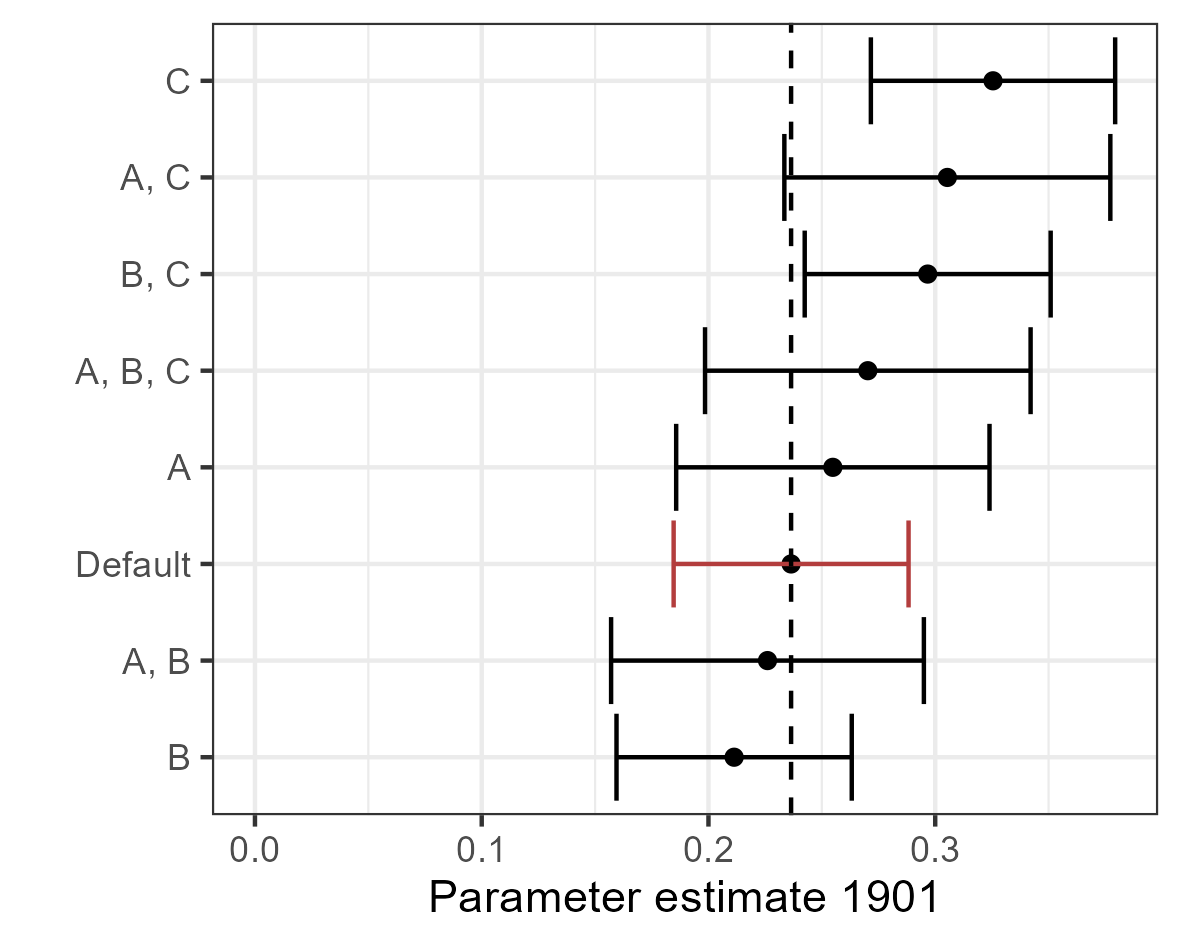
\includegraphics[width=\textwidth]{Plots/Regression_plots/Multiverse_dummy.png}
    \end{subfigure}
    \hfill
    \begin{subfigure}[b]{0.45\textwidth}
        \centering
        \caption{\label{fig:mult2} Multiverse of control groups\\Market access approach}
        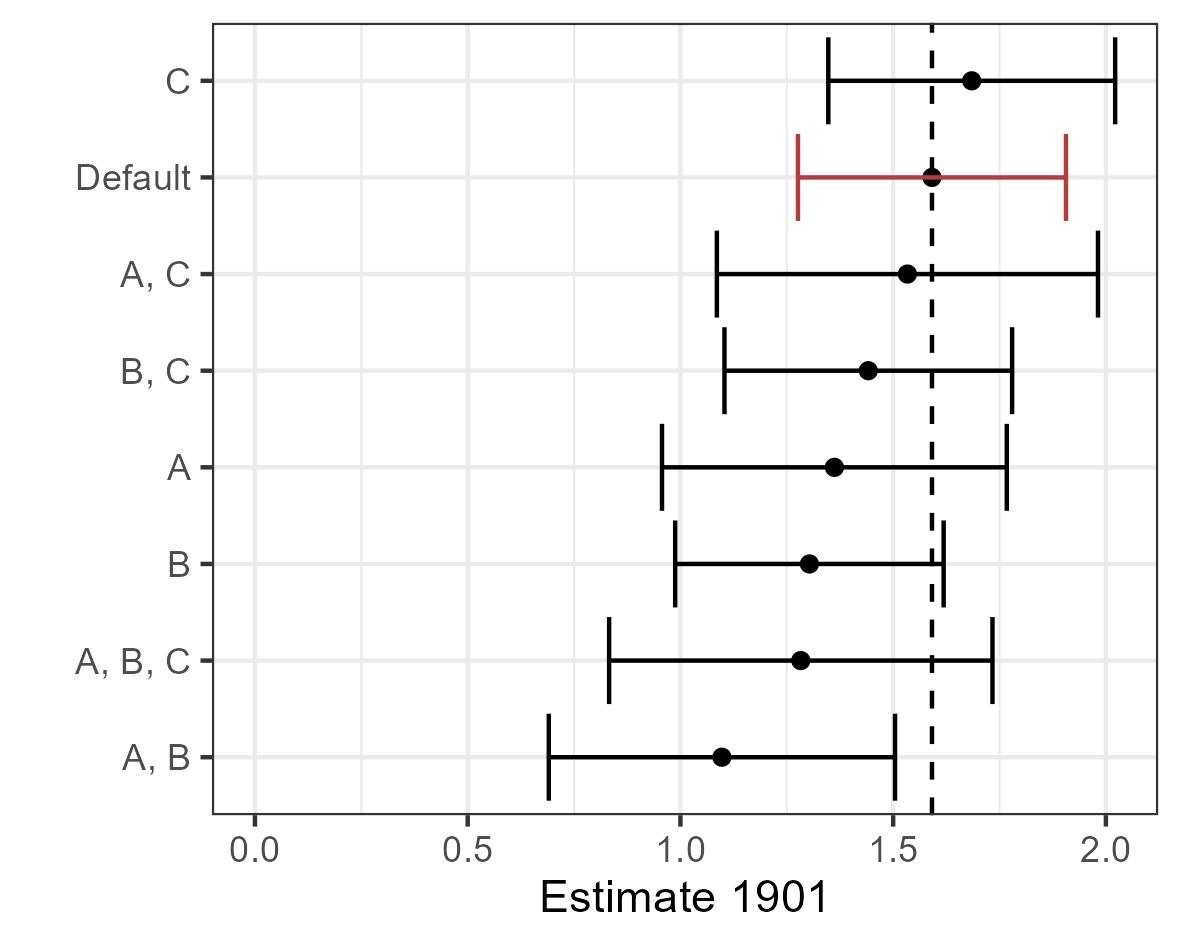
\includegraphics[width=\textwidth]{Plots/Regression_plots/Multiverse_MA.png}
    \end{subfigure}
    \vspace{0.45cm}
    \begin{subfigure}[b]{0.45\textwidth}
        \centering
        \caption{\label{fig:mult3} Multiverse of feasible parameters\\Market access approach}
        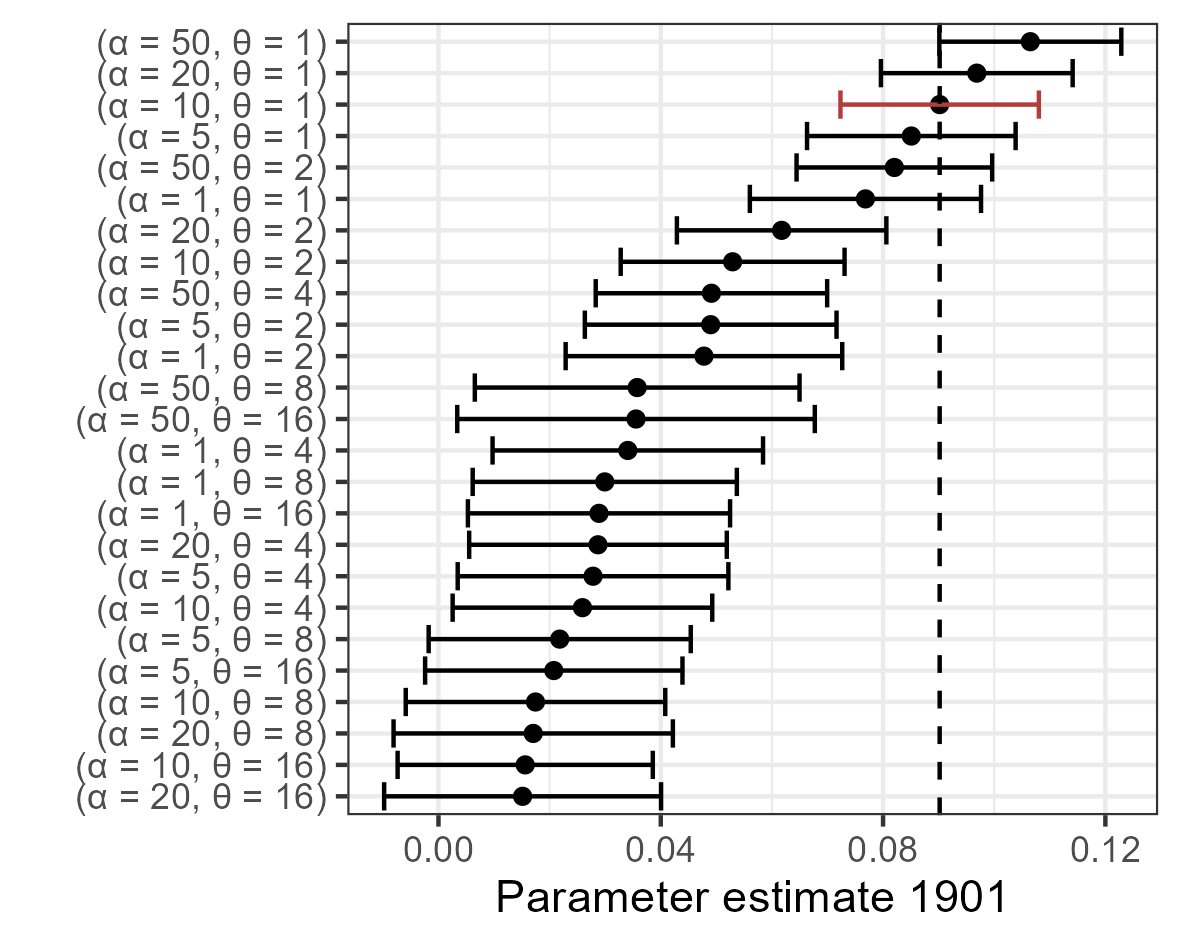
\includegraphics[width=\textwidth]{Plots/Regression_plots/Multiverse_MA_param.png}
    \end{subfigure}
    \parbox{0.9\textwidth}{
    \caption*{\footnotesize \textit{Notes:} This is the multiverse of parameter estimates of the effect in 1901 given different feasible choices that could have been made for how to run the analysis. In panel a and panel b, 'A', 'B', and 'C', represents subgroups of the data. 'A' is the result, when the regression is computed using only parishes with a centroid less than 5 km from the coast. 'B' is the subgroups, where all parishes in around Copenhagen are excluded, 'C' is the subgroup of parishes, where the control group does not contain any parishes within 100 km of the Limfjord. 'D' represents the result when using only parishes located within 5 km of a market town. Panel (c) represents the effect given different market access parameters. For enhanced comparability, the log change in market access is standardized to unit variance and zero mean. \\ \textit{Source: Danish census data}}
} \label{fig:pop2}
\end{figure}

\begin{figure}[H]
    \centering
    \caption{Multiverse of the effect in different comparison groups and parameter choices}
    \begin{subfigure}[b]{0.45\textwidth}
        \centering
        \caption{\label{fig:mult1} Multiverse of control groups\\Dummy approach}
        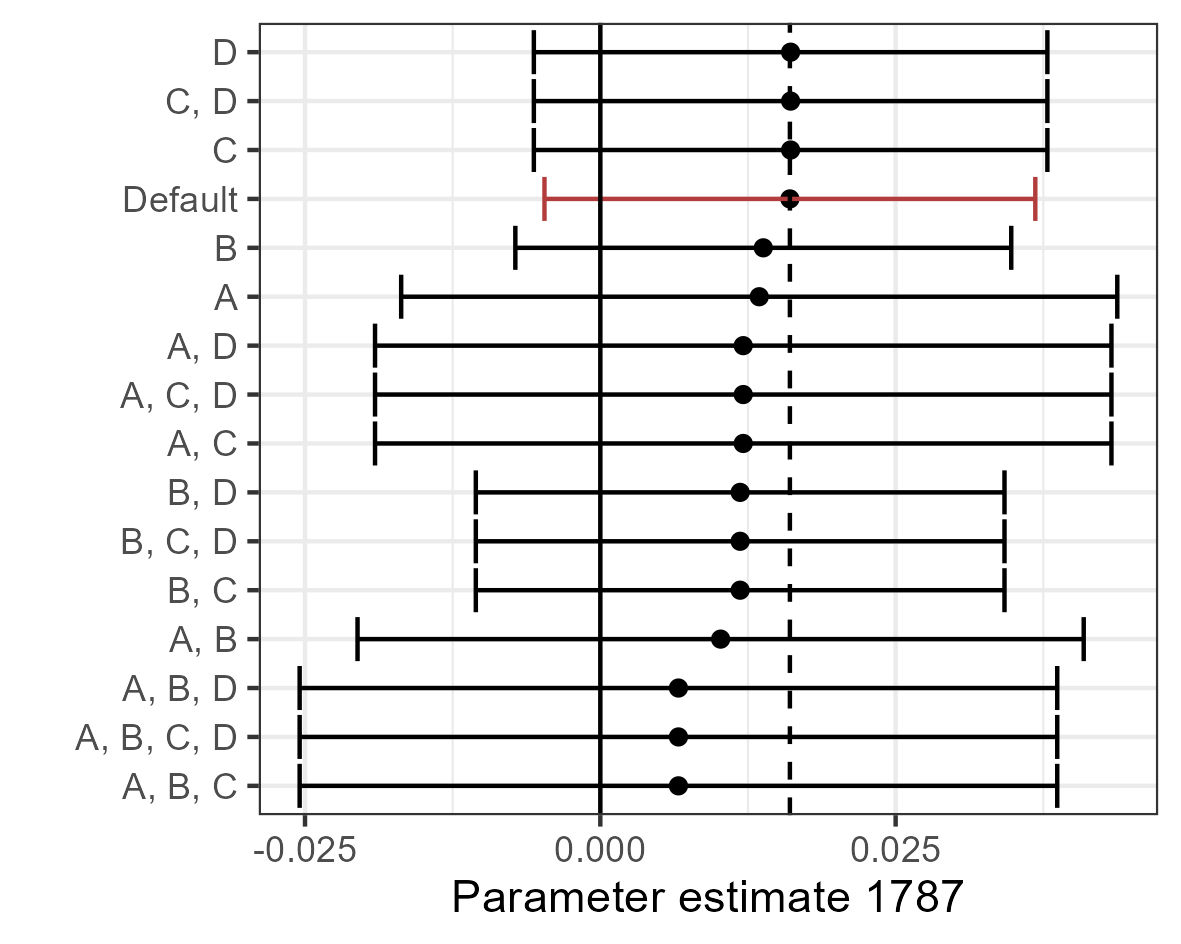
\includegraphics[width=\textwidth]{Plots/Regression_plots/Multiverse_dummy_1787.png}
    \end{subfigure}
    \hfill
    \begin{subfigure}[b]{0.45\textwidth}
        \centering
        \caption{\label{fig:mult2} Multiverse of control groups\\Market access approach}
        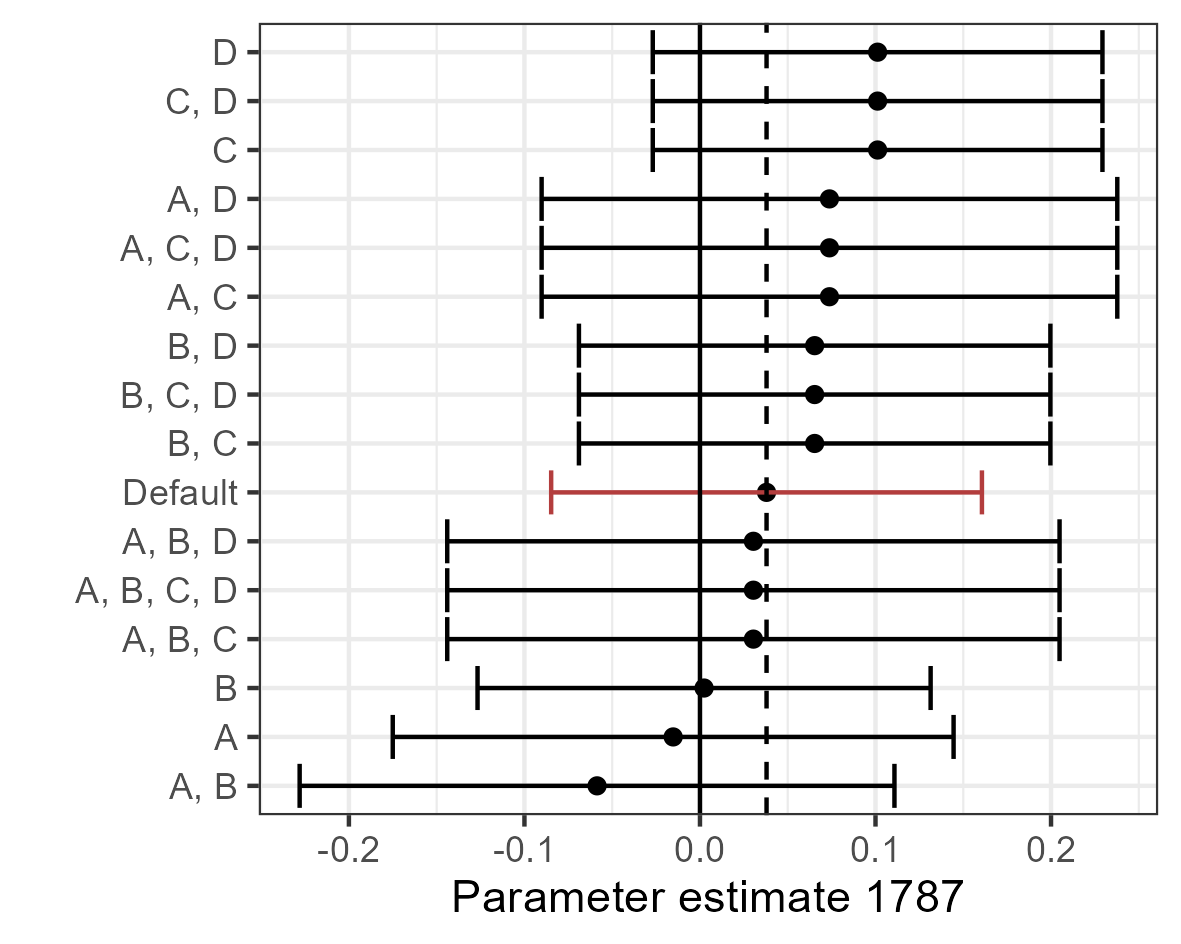
\includegraphics[width=\textwidth]{Plots/Regression_plots/Multiverse_MA_1787.png}
    \end{subfigure}
    \vspace{0.45cm}
    \begin{subfigure}[b]{0.45\textwidth}
        \centering
        \caption{\label{fig:mult3} Multiverse of feasible parameters\\Market access approach}
        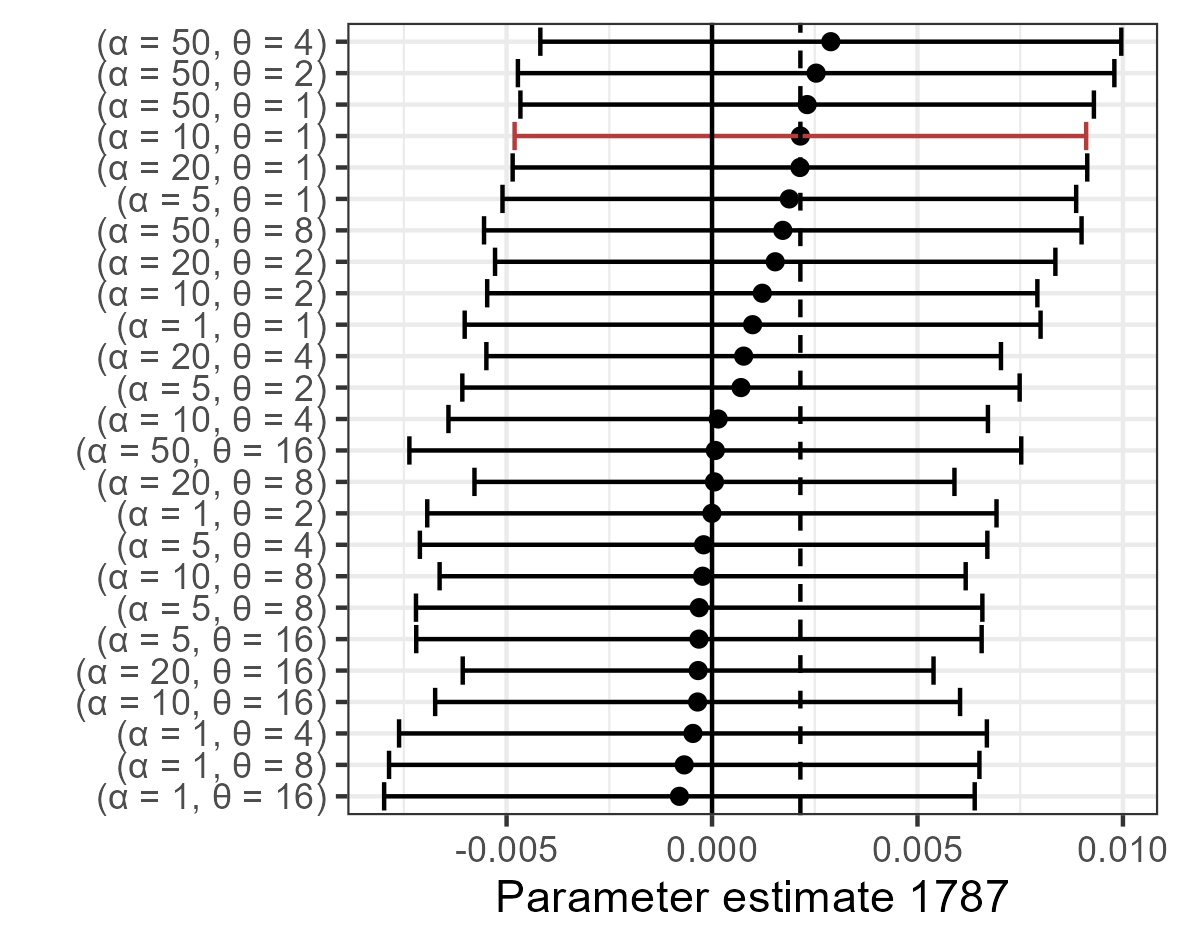
\includegraphics[width=\textwidth]{Plots/Regression_plots/Multiverse_MA_param_1787.png}
    \end{subfigure}
    \caption*{Notes: Multiverse results for 1787. If any of these were different from zero it would indicate the existence of pretends. The dotted line indicate the default parameter estimate. The solid line is at zero.}
    \label{fig:pop2}
\end{figure}

\FloatBarrier
\subsection{Doubly robust estimates}
This section contains estimates based on the doubly-robust multi-period did estimator from \cite{Callaway2021did}. Table \ref{tab:cs_estimates} shows the results. As is default in their implementation, the first period is the reference. As consequence, the reference year here is 1787 rather than 1801 from the rest of my paper. To address concern over balance, covariates are included. The doubly robust method combines a propensity score and an outcome regression and is consistent if either of these are correctly specified \citep{Santanna2020DRDID}. Column 1 shows results without covariates. Column 2 shows results including covariates (Occupation, Young children per woman and number of people in different age groups). Column 3 also includes the pre-event population as a covariate. 


\begin{table}[H]
\centering
\caption{\label{tab:cs_estimates} Callaway and Sant'Anna estimates}
\footnotesize
\begin{tabular}{lccc}
   \tabularnewline \midrule \midrule
   Outcome: & \multicolumn{3}{c}{log(Population)}\\
            & (1)           & (2)             & (3)\\  
   \midrule
    1801 & -0.0152      & -0.0273     & -0.0273 \\
         & (0.0114)     & (0.0141)    & (0.0133) \\
    1834 & 0.0221       & 0.0041      & 0.0041 \\
         & (0.0133)     & (0.0148)    & (0.0145) \\
    1840 & 0.0004       & -0.0097     & -0.0097 \\
         & (0.0132)     & (0.0154)    & (0.0145) \\
    1845 & 0.0031       & -0.0058     & -0.0058 \\
         & (0.0137)     & (0.0156)    & (0.0149) \\
    1850 & 0.0076       & -0.0040     & -0.0040 \\
         & (0.0146)     & (0.0174)    & (0.0160) \\
    1860 & 0.0343       & 0.0087      & 0.0087 \\
         & (0.0166)     & (0.0187)    & (0.0194) \\
    1880 & 0.1336*      & 0.0873*     & 0.0873* \\
         & (0.0198)     & (0.0229)    & (0.0233) \\
    1901 & 0.2262*      & 0.1590*     & 0.1590* \\
         & (0.0263)     & (0.0276)    & (0.0310)\\  
   \midrule
   Observations & 14,2741 & 14,274 & 14,274\\
   \midrule \midrule
   \multicolumn{4}{l}{\emph{'*' confidence band (95 percent) does not cover 0}}\\
\end{tabular}
\parbox{0.6\textwidth}{
\caption*{Notes: Effect using the estimator proposed by Callaway \& Sant’Anna (2021). Column (1) includes no covariates. Column (2) adjusts for pre-event covariates. Column (3) adjusts for pre-event covariates including pre-event population. \\ \textit{Source: Danish census data}}
}

\end{table}

\section{Mechanims}

\FloatBarrier
\subsection{All occupational major categories estimates} 
\begin{table}[]
    \centering
    \caption{\label{tab:occ1} Effect on occupation in 1901 (HISCO first digit 1 to 3)}
    \footnotesize
    \begin{tabular}{ccccc}
\toprule
hisco & Affected & Approach & Estimate (1901) & n parishes\\
\midrule
0/1 & MA & 3: log(x+1) & -0.642 (0.337) & 1589\\
0/1 & MA & 4: asinh(x) & -0.595 (0.397) & 1589\\
0/1 & MA & 1: Extensive & 0.414 (0.139) & 1589\\
0/1 & MA & 2: Intensive & -0.41 (0.445) & 1342\\
0/1 & Dummy & 3: log(x+1) & -0.083 (0.06) & 1589\\
0/1 & Dummy & 4: asinh(x) & -0.081 (0.07) & 1589\\
0/1 & Dummy & 1: Extensive & 0.064 (0.025) & 1589\\
0/1 & Dummy & 2: Intensive & -0.047 (0.079) & 1342\\
2 & MA & 3: log(x+1) & -0.871 (0.463) & 1589\\
2 & MA & 4: asinh(x) & -0.561 (0.521) & 1589\\
2 & MA & 1: Extensive & 0.182 (0.148) & 1589\\
2 & Dummy & 3: log(x+1) & -0.085 (0.085) & 1589\\
2 & Dummy & 2: Intensive & 0.081 (0.148) & 764\\
2 & Dummy & 4: asinh(x) & -0.056 (0.096) & 1589\\
2 & MA & 2: Intensive & 0.04 (0.761) & 764\\
2 & Dummy & 1: Extensive & -0.015 (0.025) & 1589\\
3 & MA & 2: Intensive & 1.962 (4.096) & 75\\
3 & Dummy & 2: Intensive & 1.252 (0.472) & 75\\
3 & MA & 1: Extensive & 1.128*** (0.259) & 1589\\
3 & MA & 4: asinh(x) & 0.697 (0.479) & 1589\\
3 & MA & 3: log(x+1) & 0.486 (0.381) & 1589\\
3 & Dummy & 1: Extensive & 0.169*** (0.044) & 1589\\
3 & Dummy & 4: asinh(x) & 0.101 (0.087) & 1589\\
3 & Dummy & 3: log(x+1) & 0.073 (0.07) & 1589\\
\bottomrule
\end{tabular}
\parbox{0.9\textwidth}{
\caption*{\footnotesize \textit{Notes:} Parameter estimate of the effect on occupational structure of the channel in 1901. Each row corresponds to a sepperate regression with all individuals with hisco codes starting with 0/1, 2 or 3 as outcome. The last column shows the number of parishes included in the regression, which is different from the full sample (1589) in the intensive margin estimates. As a rule of thumb, results with fewer than 100 observations should be entirely disregarded. *** $p< 0.01$ ** $p< 0.05$ * $p< 0.10$. Standard errors clustered on the parish level in parenthesis. All p-values are Bonferroni-corrected. \\ \textit{Source:} Danish census data.}
}
\end{table}

\begin{table}[]
    \centering
    \caption{\label{tab:occ2} Effect on occupation in 1901 (HISCO first digit 4 to 9)}
    \footnotesize
    \begin{tabular}{ccccc}
\toprule
hisco & Affected & Approach & Estimate (1901) & n parishes\\
\midrule
4 & MA & 2: Intensive & -4.772 (3.826) & 28\\
4 & MA & 4: asinh(x) & -1.342 (0.576) & 1589\\
4 & MA & 3: log(x+1) & -1.121 (0.489) & 1589\\
4 & Dummy & 2: Intensive & -0.353 (0.402) & 28\\
4 & Dummy & 4: asinh(x) & -0.182 (0.103) & 1589\\
4 & Dummy & 3: log(x+1) & -0.143 (0.087) & 1589\\
4 & MA & 1: Extensive & -0.123 (0.202) & 1589\\
4 & Dummy & 1: Extensive & -0.058 (0.036) & 1589\\
5 & MA & 4: asinh(x) & -0.943 (0.554) & 1589\\
5 & MA & 1: Extensive & -0.662*** (0.163) & 1589\\
5 & MA & 3: log(x+1) & -0.625 (0.462) & 1589\\
5 & Dummy & 2: Intensive & 0.309 (0.159) & 660\\
5 & MA & 2: Intensive & 0.302 (0.881) & 660\\
5 & Dummy & 3: log(x+1) & 0.057 (0.079) & 1589\\
5 & Dummy & 4: asinh(x) & 0.042 (0.094) & 1589\\
5 & Dummy & 1: Extensive & -0.031 (0.028) & 1589\\
6 & MA & 2: Intensive & 1.173*** (0.196) & 1545\\
6 & MA & 1: Extensive & -0.243*** (0.049) & 1589\\
6 & Dummy & 2: Intensive & 0.197*** (0.031) & 1545\\
6 & MA & 4: asinh(x) & -0.123 (0.322) & 1589\\
6 & Dummy & 3: log(x+1) & 0.085 (0.036) & 1589\\
6 & Dummy & 4: asinh(x) & 0.072 (0.038) & 1589\\
6 & MA & 3: log(x+1) & 0.025 (0.294) & 1589\\
6 & Dummy & 1: Extensive & -0.024*** (0.004) & 1589\\
7/8/9 & MA & 2: Intensive & 1.763*** (0.339) & 1530\\
7/8/9 & MA & 4: asinh(x) & 0.813 (0.39) & 1589\\
7/8/9 & MA & 3: log(x+1) & 0.709 (0.358) & 1589\\
7/8/9 & MA & 1: Extensive & -0.218*** (0.05) & 1589\\
7/8/9 & Dummy & 2: Intensive & 0.215** (0.063) & 1530\\
7/8/9 & Dummy & 4: asinh(x) & 0.123 (0.068) & 1589\\
7/8/9 & Dummy & 3: log(x+1) & 0.11 (0.063) & 1589\\
7/8/9 & Dummy & 1: Extensive & -0.02 (0.007) & 1589\\
\bottomrule
\end{tabular}
\parbox{0.9\textwidth}{
\caption*{\footnotesize \textit{Notes:} Parameter estimate of the effect on occupational structure of the channel in 1901. Each row corresponds to a sepperate regression with all individuals with hisco codes starting with 4, 5, or 6/8/9 as outcome. The last column shows the number of parishes included in the regression, which is different from the full sample (1589) in the intensive margin estimates. As a rule of thumb, results with fewer than 100 observations should be entirely disregarded. *** $p< 0.01$ ** $p< 0.05$ * $p< 0.10$. Standard errors clustered on the parish level in parenthesis. All p-values are Bonferroni-corrected. \\ \textit{Source:} Danish census data.}
}
\end{table}

\FloatBarrier

\subsection{Event plot fishing and spinning}
\begin{figure}[h!]
    \centering
    \caption{Fishermen and Spinners, Weavers, Knitters, Dyers And Related Workers}
    \begin{subfigure}[b]{0.45\textwidth}
        \centering
        \caption{\label{fig:migr} Fishermen (MA approach)}
        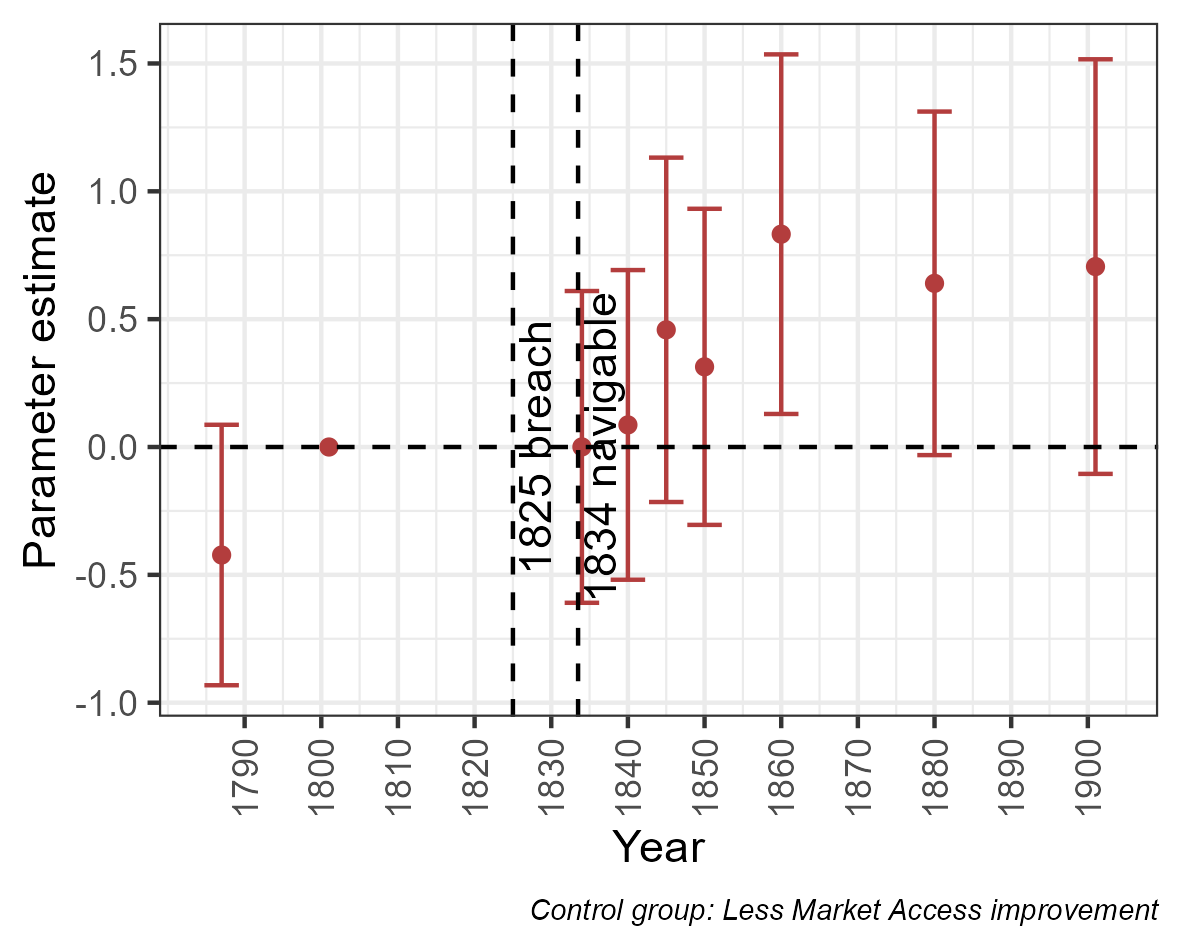
\includegraphics[width=\textwidth]{Plots/Mechanism/fish_MA.png}
    \end{subfigure}
    \hfill
    \begin{subfigure}[b]{0.45\textwidth}
        \centering
        \caption{\label{fig:fert} Fishermen (Dummy approach)}
        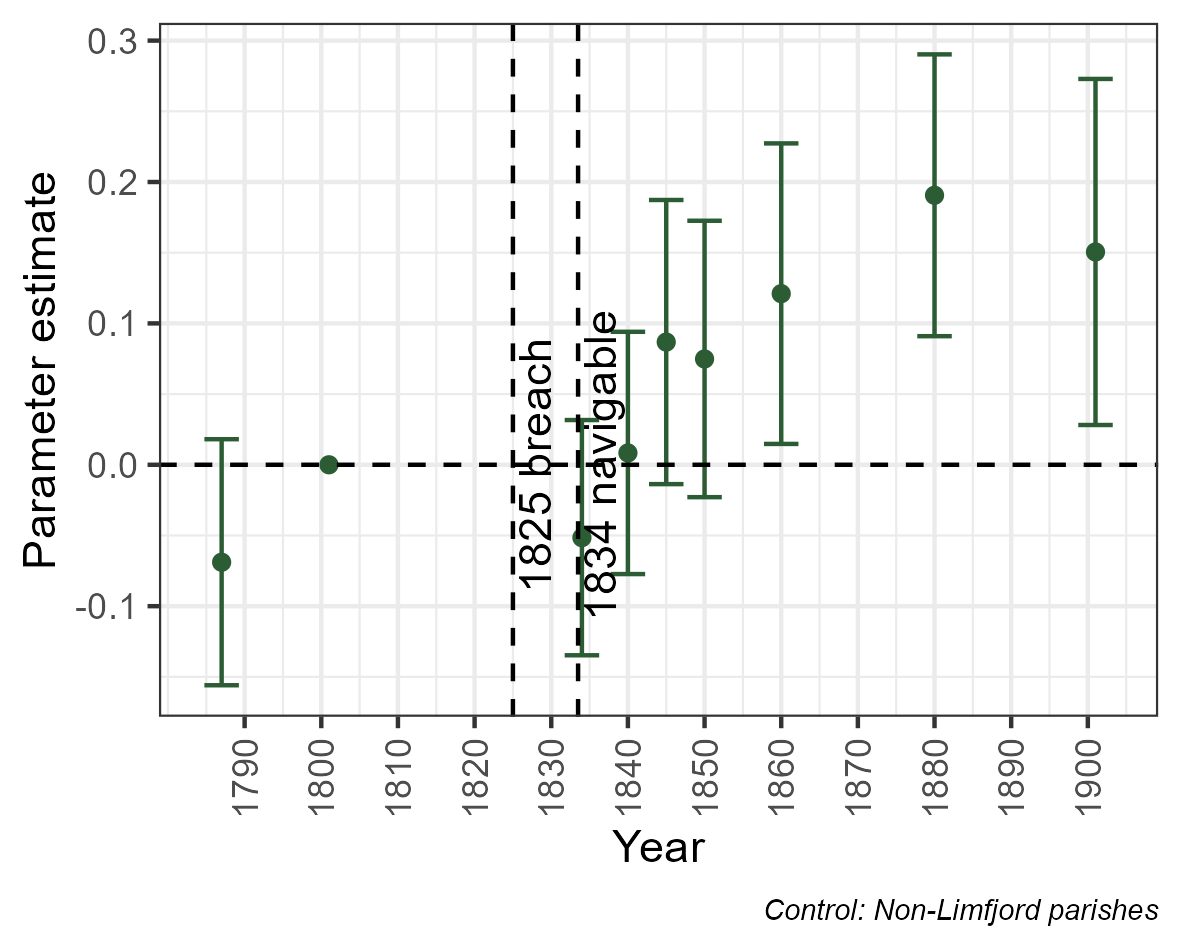
\includegraphics[width=\textwidth]{Plots/Mechanism/fish_dummy.png}
    \end{subfigure}
    \vspace{0.45cm}
    \begin{subfigure}[b]{0.45\textwidth}
        \centering
        \caption{\label{fig:migr} Spinners, weavers, knitters, dyers and related workers (MA approach)}
        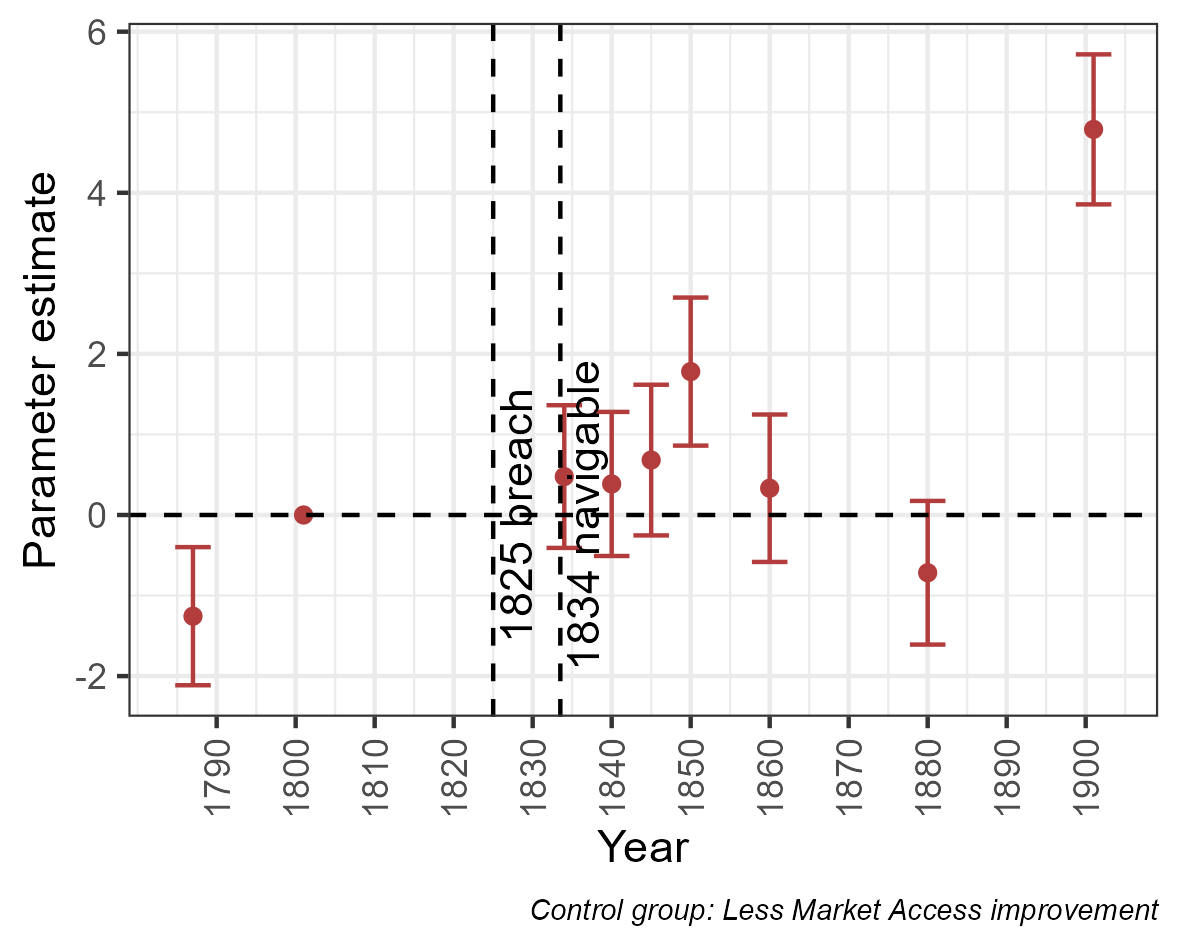
\includegraphics[width=\textwidth]{Plots/Mechanism/spinning_MA.png}
    \end{subfigure}
    \hfill
    \begin{subfigure}[b]{0.45\textwidth}
        \centering
        \caption{\label{fig:fert} Spinners, weavers, knitters, dyers and related workers (Dummy approach)}
        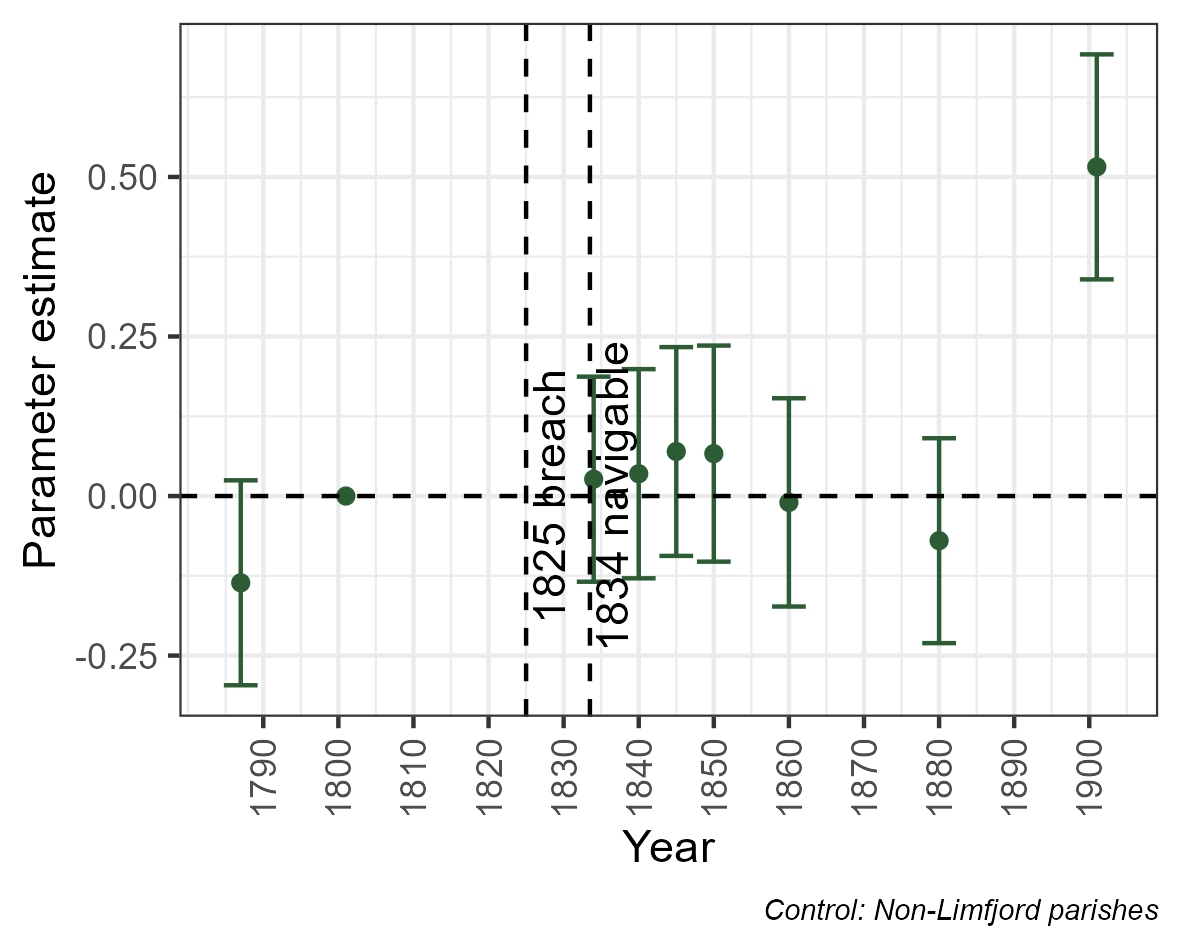
\includegraphics[width=\textwidth]{Plots/Mechanism/spinning_dummy.png}
    \end{subfigure}
    \parbox{0.9\textwidth}{
    \caption*{\footnotesize \textit{Notes:} Panel (a) and panel (b) shows event plots for the effect of the channel on the number of fishermen. Panel (c) and (d) shows the effect to the number of spinners, weavers, knitters, dyers and related workers (HISCO codes starting with 75).  \\ \textit{Source: Danish census data}}
}
    \label{fig:fishing_spinners}
\end{figure}

\FloatBarrier
\subsection{Effects by age group} 
\begin{figure}[h!]
    \centering
    \caption{Age group composition}
    \begin{subfigure}[b]{0.45\textwidth}
        \centering
        \caption{\label{fig:migr} Effect by age group (MA approach)}
        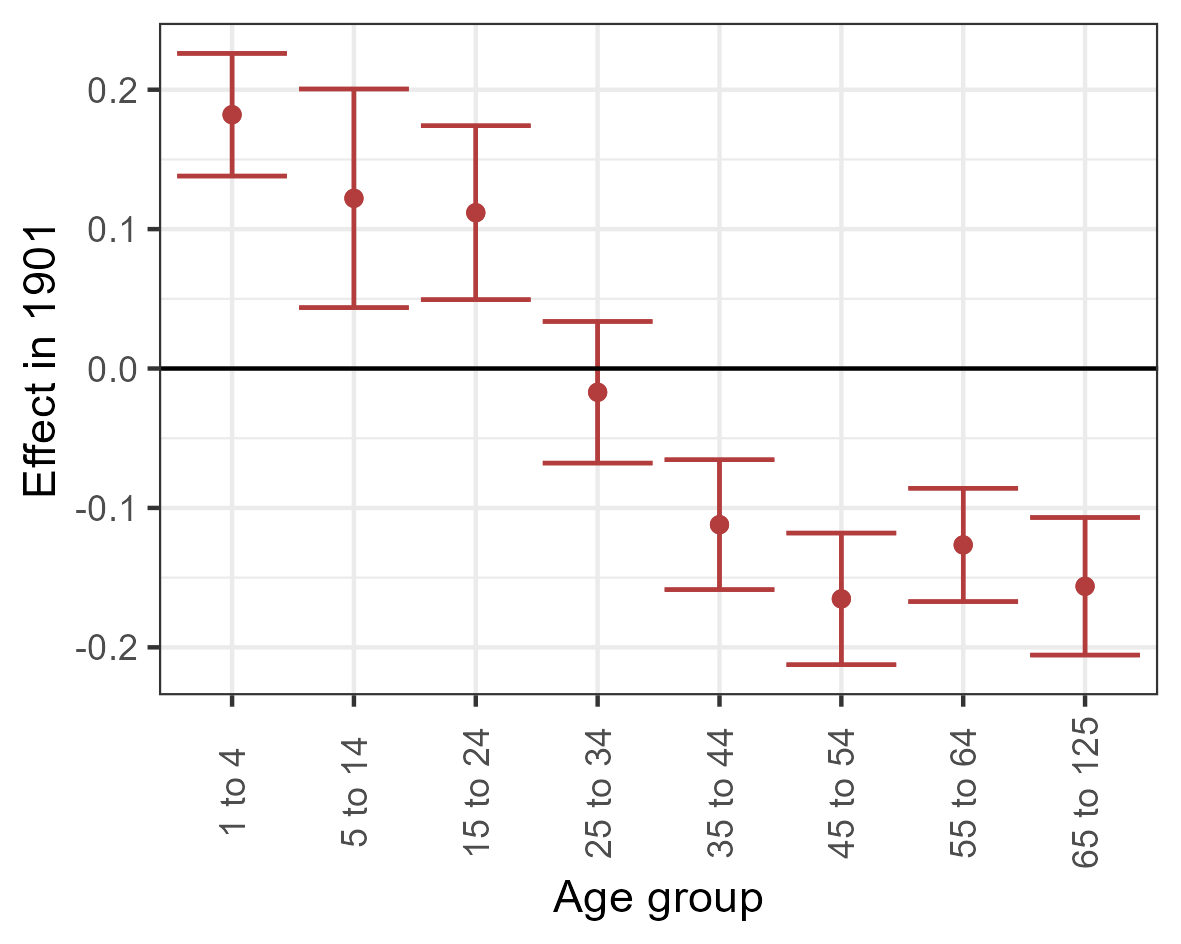
\includegraphics[width=\textwidth]{Plots/Mechanism/Age_composition_MA.png}
    \end{subfigure}
    \hfill
    \begin{subfigure}[b]{0.45\textwidth}
        \centering
        \caption{\label{fig:fert} Effect by age group (dummy approach)}
        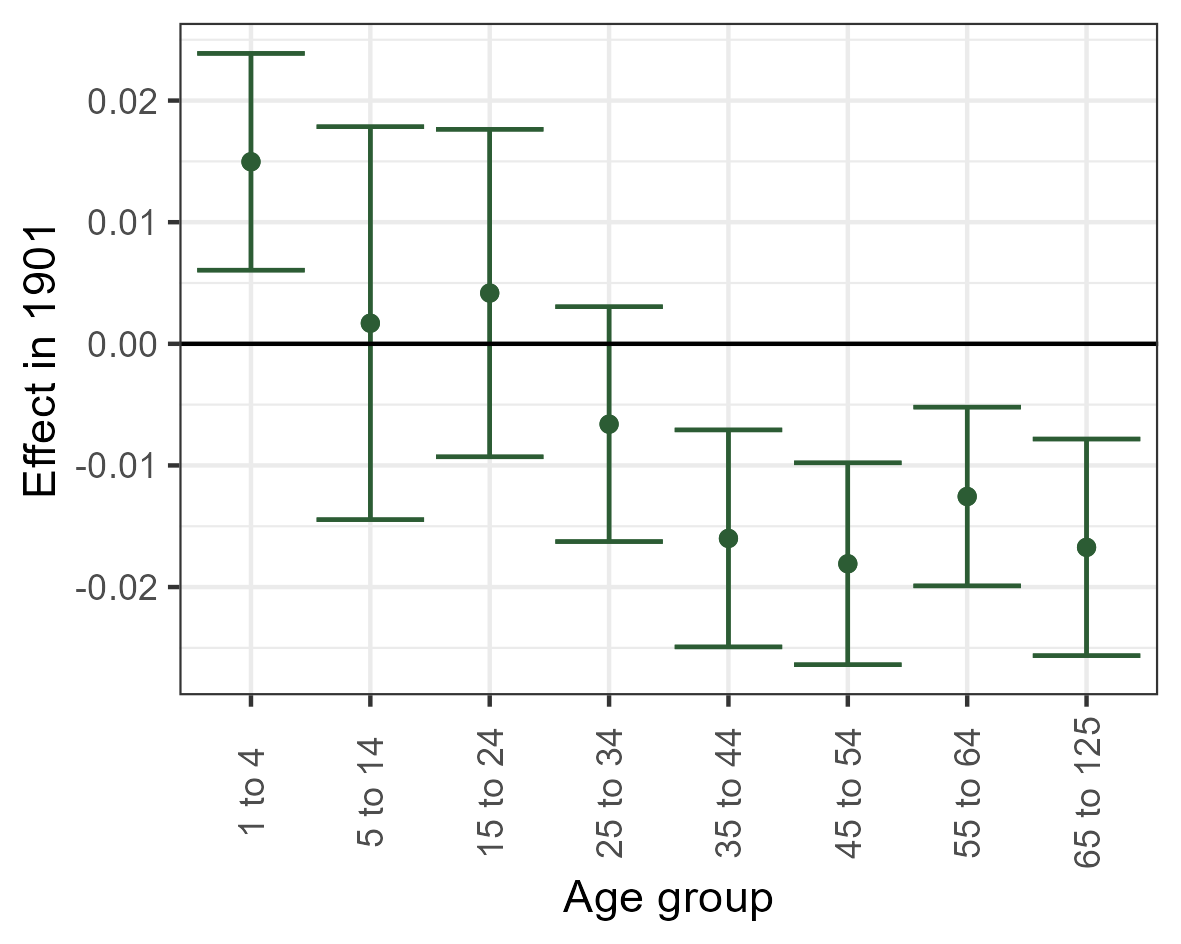
\includegraphics[width=\textwidth]{Plots/Mechanism/Age_composition_Dummy.png}
    \end{subfigure}
    \parbox{0.9\textwidth}{
    \caption*{\footnotesize \textit{Notes:} Regression parameter in 1901 given the market access approach (panel a) and the dummy approach (panel b). The outcome of each regression is the size of the particular age group as a share of the total population. What this shows, is that the population in the affected parishes became comparatively younger.  \\ \textit{Source: Danish census data}}
}
    \label{fig:age_group}
\end{figure}

\FloatBarrier
\section{Archaeological findings}

\subsection{Math note} 
The derivation is based on a single parish $i$. To construct a panel this is simply repeated for all parishes. The derivation is based on coin findings. But it generalises to any kind of finding.    

The data is of the form: $Coin=c$ was generated in time interval $t\in [Y_{min}^c;Y_{max}^c]$ (Archaeologists report a coin finding and date it to a range.)

That is, for each coin we observe $P(t|c)\sim [Y_{min}^c;Y_{max}^c]$ 

We want to know the probability, that any coin, $c\in \{1, ..., K\}$, finding was generated at any particular point in time. This event is referred to as $\{coins\}|t$

\subsubsection{Probability of a single coin} 
We are interested in the probability that a any coin comes from a specific point in time. What is observed is:

\begin{equation}
P(t|c)=\begin{cases}
\frac{1}{Y_{max}^c - Y_{min}^c}, & \text{if }Y_{min}^c\leq t \leq Y_{max}^c \\
0 & \text{otherwise}
\end{cases}
\end{equation}

Or writing the same with indicator function:

\begin{equation}
P(t|c)=1[t\in [Y_{min}^c;Y_{max}^c]]\frac{1}{Y_{max}^c - Y_{min}^c}
\end{equation}

I.e. it is equally likely that a coin truly originates at any particular point in time the range offered by the archaeologists. 

**Note:**
This is an assumption. The archaeologists specify a range but not a distribution. How should this range be interpreted? A straightforward alternative is to intepret it as a 95 percent confidence interval of the normal distribution. This is also tested. 

\begin{equation}
\begin{split}
P(t|c)&=\mathcal{N}(\mu_c,\sigma_c)\\
\text{where:} \\
\mu_c&=0.5\times(Y_{max}^c + Y_{min}^c)\\
\sigma_c&\approx(Y_{max}^c - Y_{min}^c)/1.96
\end{split}
\end{equation}

\subsubsection{At the parish level}
The probability that *any* coin was generated as a finding in the parish (at least one of the draws from $P(t|c)$ was succesful) is a mixture distribution, where at least one component needs to be sucesful:

\begin{equation}
\begin{split}
P(t|\{coins\})&=1-\prod_{c=1}^K \left( 1 - P(t|c) \right) \\
P(t|\{coins\})&=1-\prod_{c=1}^K \left(1 - 1[t\in [Y_{min}^c;Y_{max}^c]] \left(\frac{1}{Y_{max}^c - Y_{min}^c}\right) \right)
\end{split}
\end{equation}

where $\{coins\}$ is the event of at least one coin $\{coins\}=\{1,...,c,...,K\}$. 

*Intuition*
The inner part of the expression ($1 - P(t|c)$) is the probability that a coin is *not* associated with that particular point in time. Taking the product over all coins, generates the combined probability, that *no coins at all* are associated with that particular point in time. The compliment of this is the probability we are interested in, in this step. It is the probability that *any* coin is associated with a particular point in time. 

\subsubsection{Reverse probability} 
We are interested in the reverse probability: The probability of any coins given a particular point in time. The formula for this is Bayes formula:

\begin{equation}
P(\{coins\}|t) = \frac{P(t|\{coins\})P(\{coins\})}{P(t)}
\end{equation}

The prior, $P(\{coins\})$, is simply assumed to be a constant, $0<c<1$ and $P(t)$ can be found by marginalisation  $P(t)=P(t|\{coins\})+P(t|\neg\{coins\})=1$. It follows that

\begin{equation}
P(\{coins\}|t) = c\times P(t|\{coins\})
\end{equation}

\subsubsection{Estimation}
The following loop (pseudocode) produces samples from $P(\{coins\}|t)$ and estimates the probability of interest:

```{pseudo code}
B = 1000 # Number of Monte Carlo samples

for b in 1 to B: # Loop of MC samples
	# Generate samples from Y_max_c Y_max_c:
	for c in 1 to C:
		t_c = sample_uniform(1, Y_min_c, Y_max_c)
		# Is t_c equal to t?
		coins_t[c] = t_c == t
		
	# Were there any coins associated with this time in this draw?
	number_of_coins = sum(coins_t)
	succces_t[b] = number_of_coins > 0
	
# Estimating the probability by analogy for each t
P_of_t_given_coins = sum(succces_t) / B

# Converting to P({coins}|t)
P_of_coins_given_t = c_hat * P_of_t_given_coins
```


This code is then repeated for every parish and every point in time $t$. This gives a panel of size $N\times T$ containing the estimated probability that a coin finding was generated at a particular point in time. This in turn can be used in econometric applications. 

\newpage
\subsection{All parameter estimates}
Table \ref{tab:A_arch1} and \ref{tab:A_arch2} contain parameter estimates for all years for the regressions using archaeological findings. 

\begin{table}[H]
\centering
\footnotesize
\caption{\label{tab:A_arch1} All parameters of table 3 columns 1-4}
\begin{tabular}{lcccc}
   \tabularnewline \midrule \midrule
                                                    & \multicolumn{4}{c}{Archaeological findings}\\
                                                    & (1)             & (2)             & (3)                   & (4)\\  
                                                    & MA              & Dummy           & MA                    & Dummy\\
   \midrule
   Year750 $\times$ Affected                        & 0.0521$^{***}$  & 0.0050$^{***}$  & 0.0034                & -0.0010\\   
                                                    & (0.0091)        & (0.0009)        & (0.0103)              & (0.0019)\\   
   Year800 $\times$ Affected                        & 0.0195$^{***}$  & 0.0020$^{***}$  & -0.0060               & -0.0024$^{*}$\\   
                                                    & (0.0047)        & (0.0005)        & (0.0068)              & (0.0013)\\   
   Year850 $\times$ Affected                        & 0.0220$^{***}$  & 0.0022$^{***}$  & -0.0072               & -0.0028$^{**}$\\   
                                                    & (0.0048)        & (0.0005)        & (0.0067)              & (0.0013)\\   
   Year900 $\times$ Affected                        & 0.0086$^{**}$   & 0.0010$^{***}$  & -0.0031               & -0.0014$^{*}$\\   
                                                    & (0.0034)        & (0.0004)        & (0.0041)              & (0.0008)\\   
   Year950 $\times$ Affected                        & -0.0042         & -0.0002         & 0.0011                & 0.0002\\   
                                                    & (0.0037)        & (0.0004)        & (0.0019)              & (0.0004)\\   
   Year1050 $\times$ Affected                       & 0.0059$^{**}$   & 0.0008$^{***}$  & -0.0063$^{**}$        & -0.0007\\   
                                                    & (0.0026)        & (0.0003)        & (0.0032)              & (0.0006)\\   
   Year1100 $\times$ Affected                       & 0.0077          & 0.0004          & -0.0708$^{***}$       & -0.0066$^{**}$\\   
                                                    & (0.0121)        & (0.0012)        & (0.0163)              & (0.0033)\\   
   Year1150 $\times$ Affected                       & 0.0075          & 0.0003          & -0.0681$^{***}$       & -0.0065$^{*}$\\   
                                                    & (0.0122)        & (0.0012)        & (0.0168)              & (0.0034)\\   
   Year1200 $\times$ Affected                       & -0.0327$^{**}$  & -0.0049$^{***}$ & -0.0736$^{***}$       & -0.0069$^{*}$\\   
                                                    & (0.0150)        & (0.0013)        & (0.0171)              & (0.0035)\\   
   Year1250 $\times$ Affected                       & -0.0941$^{***}$ & -0.0120$^{***}$ & -0.0772$^{***}$       & -0.0066$^{*}$\\   
                                                    & (0.0194)        & (0.0017)        & (0.0190)              & (0.0038)\\   
   Year1300 $\times$ Affected                       & -0.1479$^{***}$ & -0.0147$^{***}$ & -0.0685$^{***}$       & -0.0068$^{**}$\\   
                                                    & (0.0223)        & (0.0030)        & (0.0179)              & (0.0032)\\   
   Year1350 $\times$ Affected                       & -0.1923$^{***}$ & -0.0193$^{***}$ & -0.0612$^{***}$       & -0.0065$^{**}$\\   
                                                    & (0.0267)        & (0.0036)        & (0.0192)              & (0.0032)\\   
   Year1400 $\times$ Affected                       & -0.1207$^{***}$ & -0.0116$^{***}$ & -0.0605$^{***}$       & -0.0060$^{*}$\\   
                                                    & (0.0237)        & (0.0034)        & (0.0183)              & (0.0031)\\   
   Year1450 $\times$ Affected                       & -0.0606$^{***}$ & -0.0052         & -0.0599$^{***}$       & -0.0060$^{**}$\\   
                                                    & (0.0233)        & (0.0035)        & (0.0181)              & (0.0030)\\   
   Year1500 $\times$ Affected                       & -0.1114$^{***}$ & -0.0104$^{***}$ & -0.0666$^{***}$       & -0.0064$^{*}$\\   
                                                    & (0.0252)        & (0.0038)        & (0.0235)              & (0.0036)\\   
   \midrule \midrule
   \multicolumn{5}{l}{\emph{Custom standard-errors in parentheses}}\\
   \multicolumn{5}{l}{\emph{Signif. Codes: ***: 0.01, **: 0.05, *: 0.1}}\\
\end{tabular}
\end{table}


\begin{table}
\centering
\footnotesize
\caption{\label{tab:A_arch2} All parameters of table 3 columns 5-8}
\begin{tabular}{lcccc}
   \tabularnewline \midrule \midrule
                                                    & \multicolumn{4}{c}{Archaeological findings}\\
                                                    & (5)             & (6)             & (7)                   & (8)\\  
                                                    & MA              & Dummy           & MA                    & Dummy\\
   \midrule
   Year750 $\times$ Affected   & 0.0277$^{*}$           & 0.0033$^{*}$           & -0.0086        & -0.0026\\   
                               & (0.0141)               & (0.0018)               & (0.0179)       & (0.0024)\\   
   Year800 $\times$ Affected   & 0.0106                 & 0.0013                 & -0.0082        & -0.0020\\   
                               & (0.0073)               & (0.0010)               & (0.0144)       & (0.0021)\\   
   Year850 $\times$ Affected   & 0.0157$^{**}$          & 0.0020$^{*}$           & -0.0064        & -0.0021\\   
                               & (0.0078)               & (0.0011)               & (0.0139)       & (0.0021)\\   
   Year900 $\times$ Affected   & 0.0003                 & $6.47\times 10^{-5}$   & -0.0060        & -0.0014\\   
                               & (0.0080)               & (0.0010)               & (0.0086)       & (0.0013)\\   
   Year950 $\times$ Affected   & -0.0119                & -0.0015                & 0.0013         & $-6.47\times 10^{-5}$\\    
                               & (0.0115)               & (0.0014)               & (0.0037)       & (0.0006)\\   
   Year1050 $\times$ Affected  & 0.0002                 & $4.31\times 10^{-5}$   & -0.0092        & -0.0013\\   
                               & (0.0026)               & (0.0003)               & (0.0062)       & (0.0009)\\   
   Year1100 $\times$ Affected  & -0.0070                & -0.0009                & -0.0666$^{**}$ & -0.0066\\   
                               & (0.0142)               & (0.0018)               & (0.0321)       & (0.0050)\\   
   Year1150 $\times$ Affected  & -0.0060                & -0.0009                & -0.0649$^{**}$ & -0.0063\\   
                               & (0.0134)               & (0.0017)               & (0.0329)       & (0.0051)\\   
   Year1200 $\times$ Affected  & -0.0448$^{**}$         & -0.0060$^{**}$         & -0.0789$^{**}$ & -0.0085\\   
                               & (0.0185)               & (0.0026)               & (0.0352)       & (0.0055)\\   
   Year1250 $\times$ Affected  & -0.0854$^{***}$        & -0.0114$^{***}$        & -0.0947$^{**}$ & -0.0108$^{*}$\\   
                               & (0.0262)               & (0.0039)               & (0.0379)       & (0.0059)\\   
   Year1300 $\times$ Affected  & -0.1003$^{***}$        & -0.0104$^{**}$         & -0.0952$^{**}$ & -0.0118$^{**}$\\   
                               & (0.0307)               & (0.0048)               & (0.0393)       & (0.0057)\\   
   Year1350 $\times$ Affected  & -0.1293$^{***}$        & -0.0149$^{**}$         & -0.0839$^{**}$ & -0.0103$^{*}$\\   
                               & (0.0415)               & (0.0060)               & (0.0420)       & (0.0060)\\   
   Year1400 $\times$ Affected  & -0.0827$^{***}$        & -0.0090$^{*}$          & -0.0852$^{**}$ & -0.0101$^{*}$\\   
                               & (0.0320)               & (0.0051)               & (0.0412)       & (0.0059)\\   
   Year1450 $\times$ Affected  & -0.0532                & -0.0047                & -0.0887$^{**}$ & -0.0105$^{*}$\\   
                               & (0.0324)               & (0.0052)               & (0.0410)       & (0.0059)\\   
   Year1500 $\times$ Affected  & -0.0712$^{**}$         & -0.0067                & -0.0726        & -0.0093\\   
                               & (0.0341)               & (0.0055)               & (0.0464)       & (0.0062)\\    
   \midrule \midrule
   \multicolumn{5}{l}{\emph{Custom standard-errors in parentheses}}\\
   \multicolumn{5}{l}{\emph{Signif. Codes: ***: 0.01, **: 0.05, *: 0.1}}\\
\end{tabular}
\end{table}

\FloatBarrier
\subsection{Normal distribution}
Figure \ref{fig:arch_reg1}, \ref{fig:arch_reg_boot1}, \ref{fig:arch_reg2} and \ref{fig:arch_reg_boot2} show equivalent results to those presented in the paper. However, these are results based on assuming that the archaeological datings (e.g. coin finding dated to the years 1300-1495) represent a 95 percent confidence interval from a normal distribution rather than an uniform distribution. Figure \ref{fig:arch_reg1} shows results confidence intervals for all parameters using the full sample. Figure \ref{fig:arch_reg2} shows the same results using the matched sample. Figure \ref{fig:arch_reg_boot1} and \ref{fig:arch_reg_boot2} show all the bootstrap draws for 1350.

Note that the results are qualitatively the same as the main results. 


\begin{figure}[h!]
    \centering
    \caption{Archaelogical results (full sample)}
    \begin{subfigure}[b]{0.45\textwidth}
        \centering
        \caption{\label{fig:arch1a} Coins: Market access approach}
        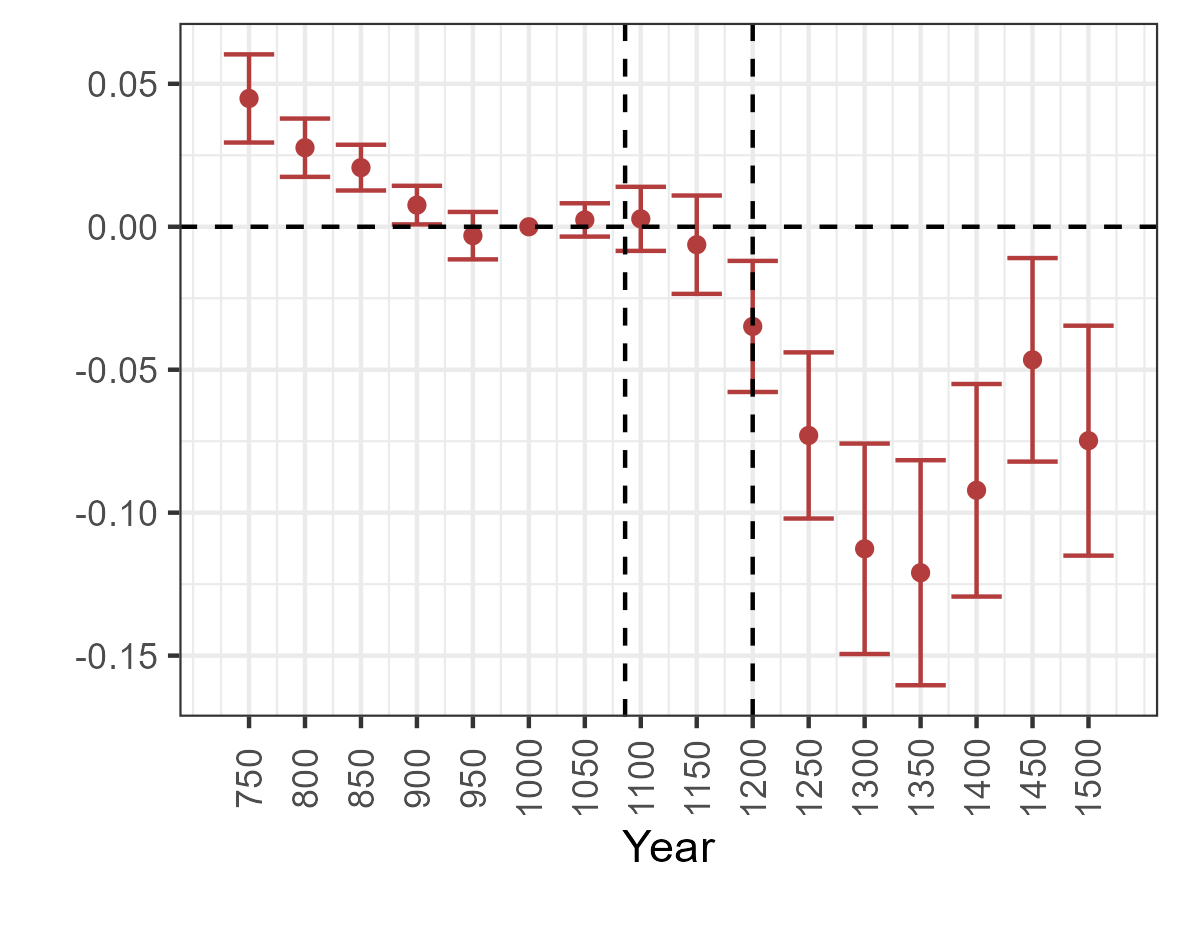
\includegraphics[width=\textwidth]{Plots/Regression_plots/arch_MA_coins_norm.png}
    \end{subfigure}
    \hfill
    \begin{subfigure}[b]{0.45\textwidth}
        \centering
        \caption{\label{fig:arch1b} Coins: Dummy approach}
        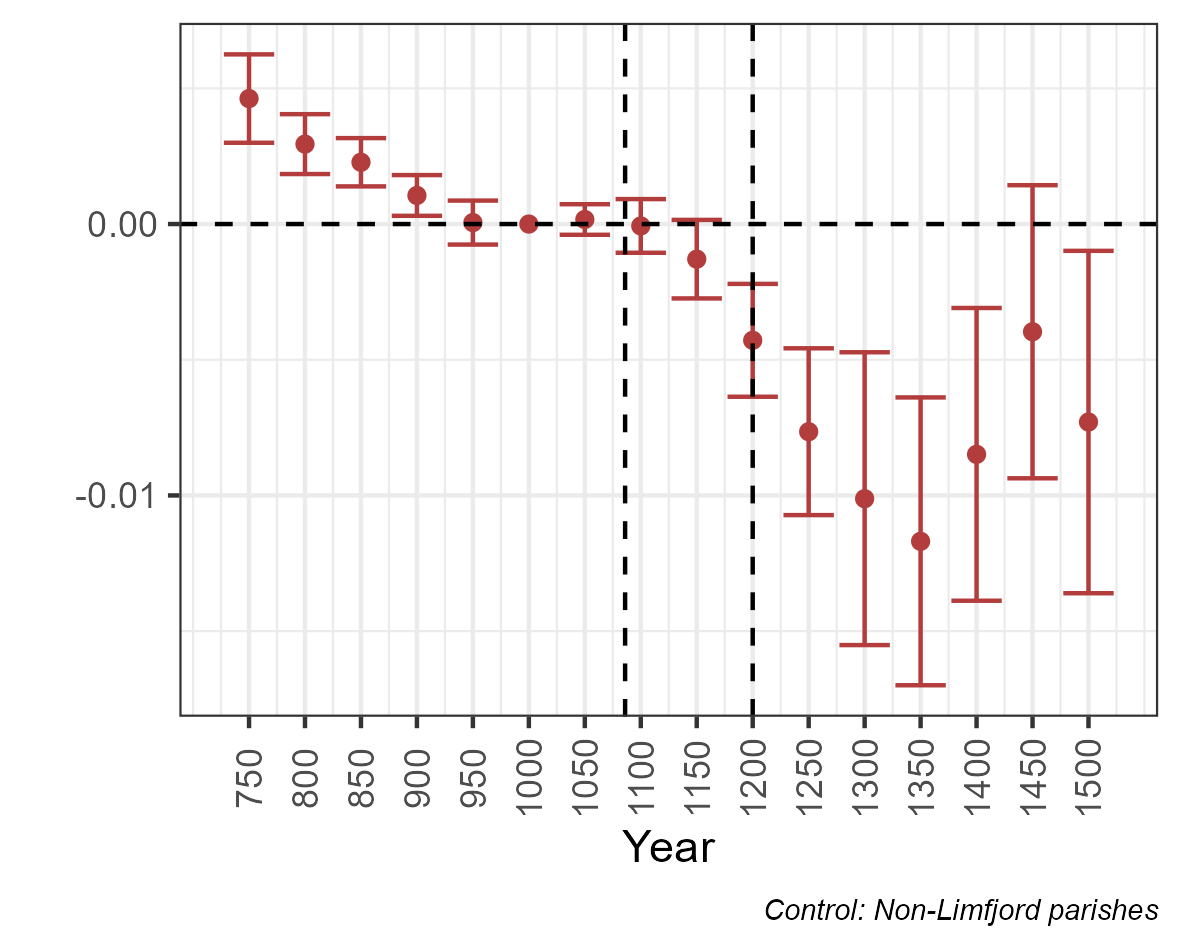
\includegraphics[width=\textwidth]{Plots/Regression_plots/arch_dummy_coins_norm.png}
    \end{subfigure}
    \vspace{0.45cm}
    \begin{subfigure}[b]{0.45\textwidth}
        \centering
        \caption{\label{fig:arch1c} Buildings: Market access approach}
        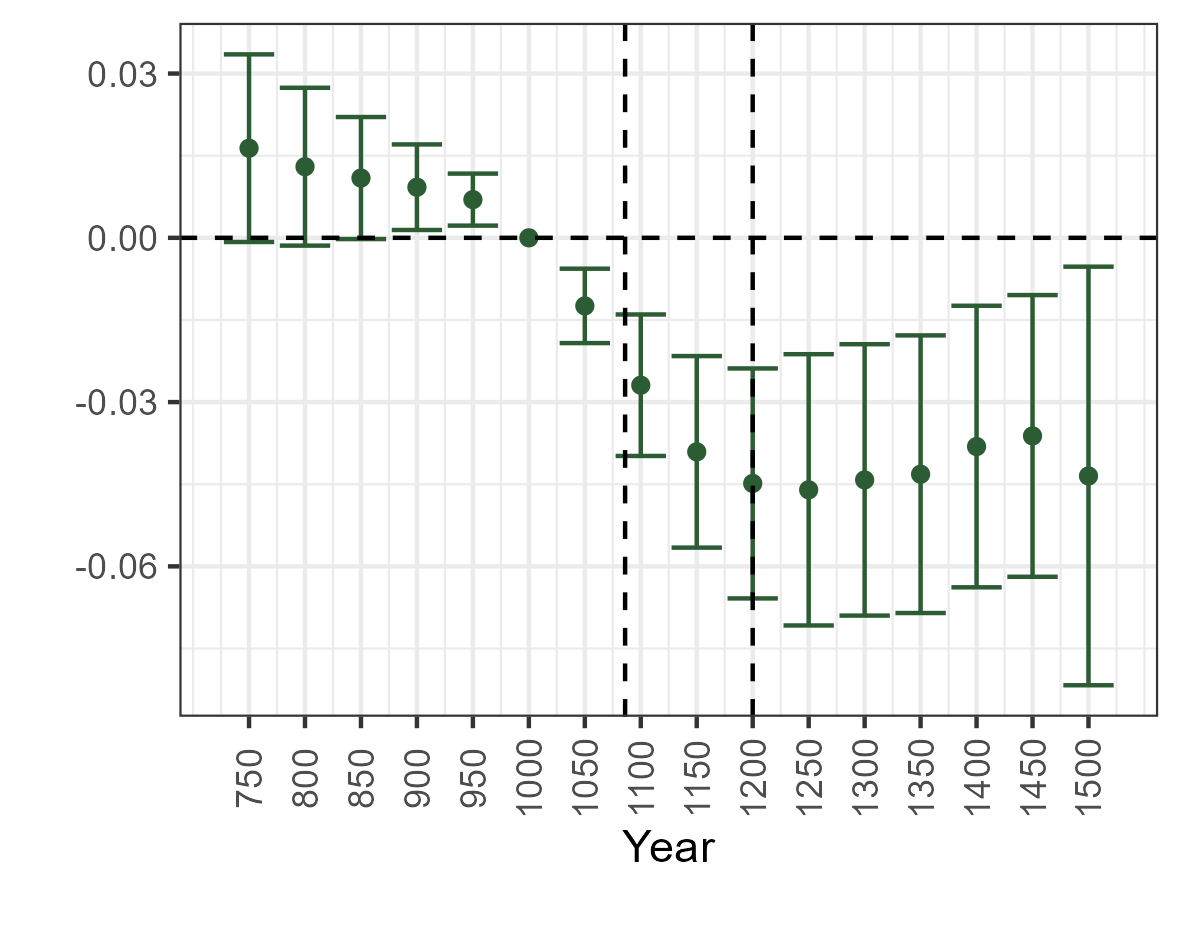
\includegraphics[width=\textwidth]{Plots/Regression_plots/arch_MA_buildings_norm.png}
    \end{subfigure}
    \hfill
    \begin{subfigure}[b]{0.45\textwidth}
        \centering
        \caption{\label{fig:arch1d} Buildings: Dummy approach}
        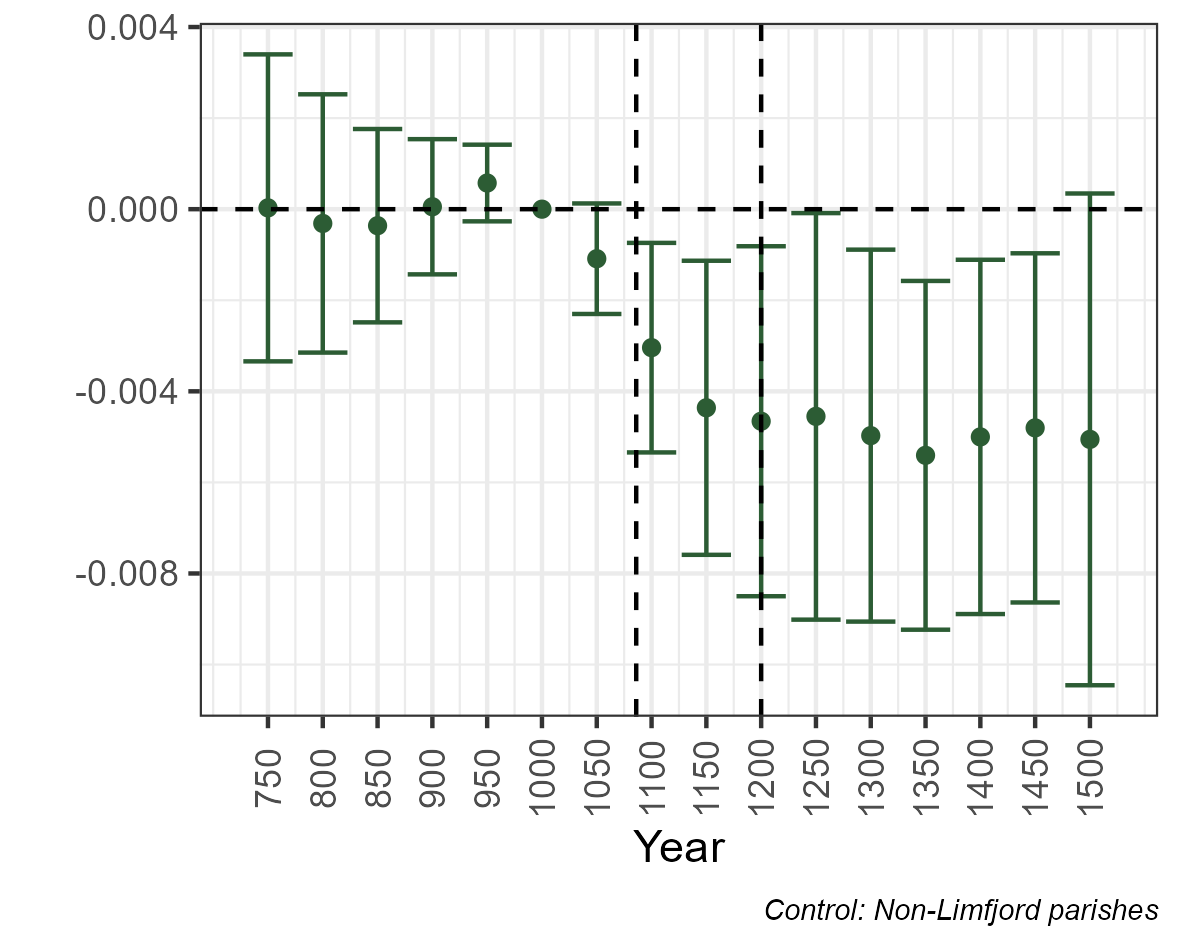
\includegraphics[width=\textwidth]{Plots/Regression_plots/arch_dummy_buildings_norm.png}
    \end{subfigure}
    \label{fig:arch_reg1}
\end{figure}


\begin{figure}[h!]
    \centering
    \caption{Distribution of parameter estimates in 1350  (full sample)}
    \begin{subfigure}[b]{0.45\textwidth}
        \centering
        \caption{\label{fig:distri_a} Coins: Market access approach}
        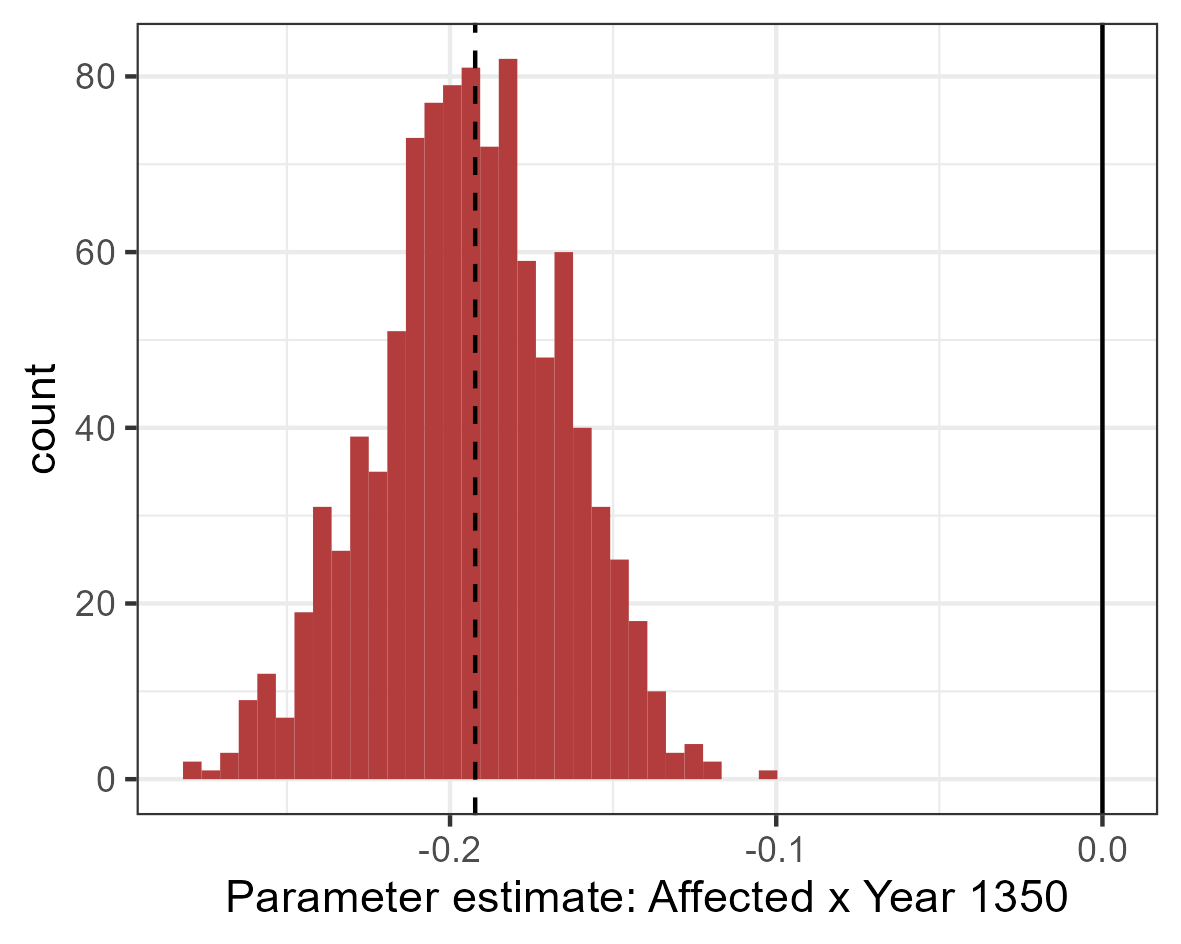
\includegraphics[width=\textwidth]{Plots/Regression_plots/arch_MA_coins_boot_norm.png}
    \end{subfigure}
    \hfill
    \begin{subfigure}[b]{0.45\textwidth}
        \centering
        \caption{\label{fig:distri_b} Coins: Dummy approach}
        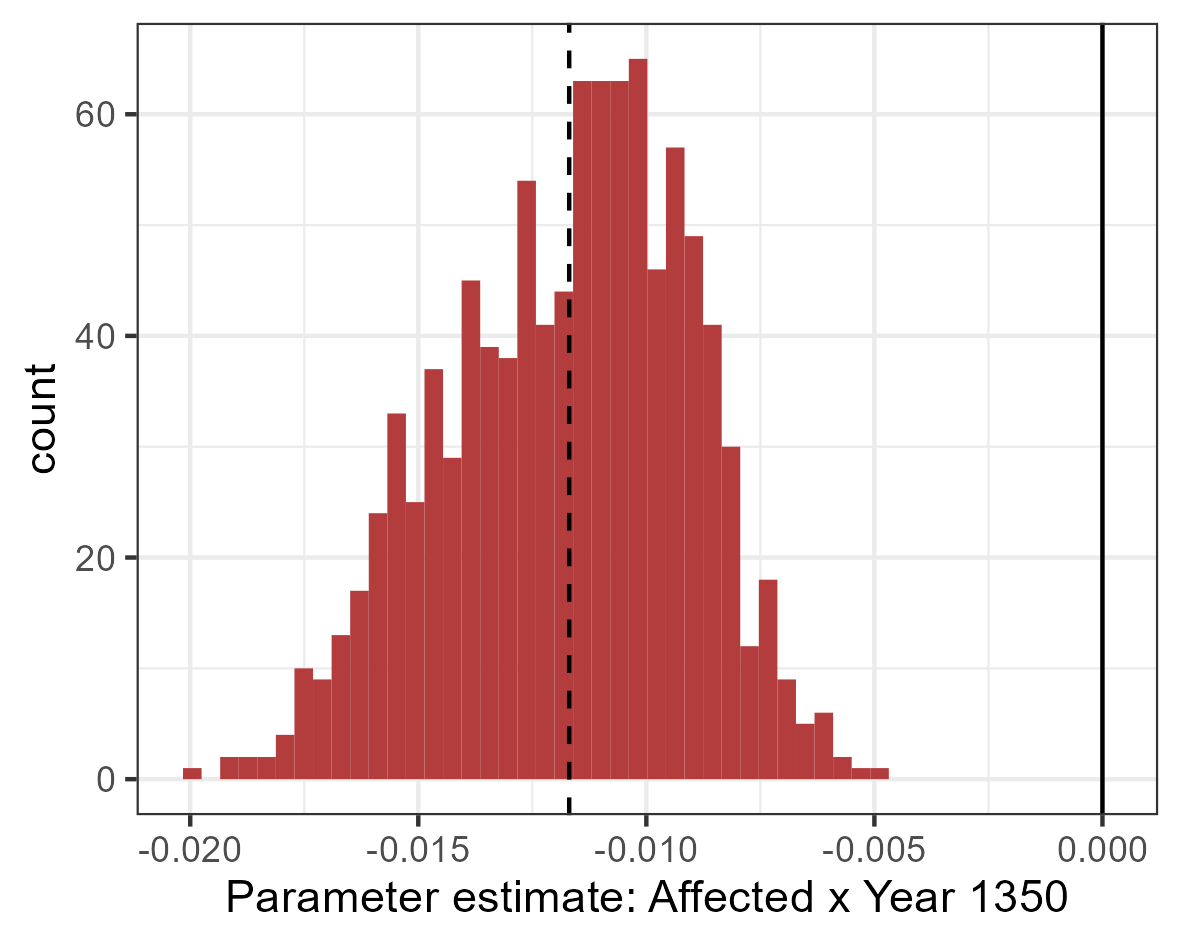
\includegraphics[width=\textwidth]{Plots/Regression_plots/arch_dummy_coins_boot_norm.png}
    \end{subfigure}
    \vspace{0.45cm}
    \begin{subfigure}[b]{0.45\textwidth}
        \centering
        \caption{\label{fig:distri_c} Buildings: Market access approach}
        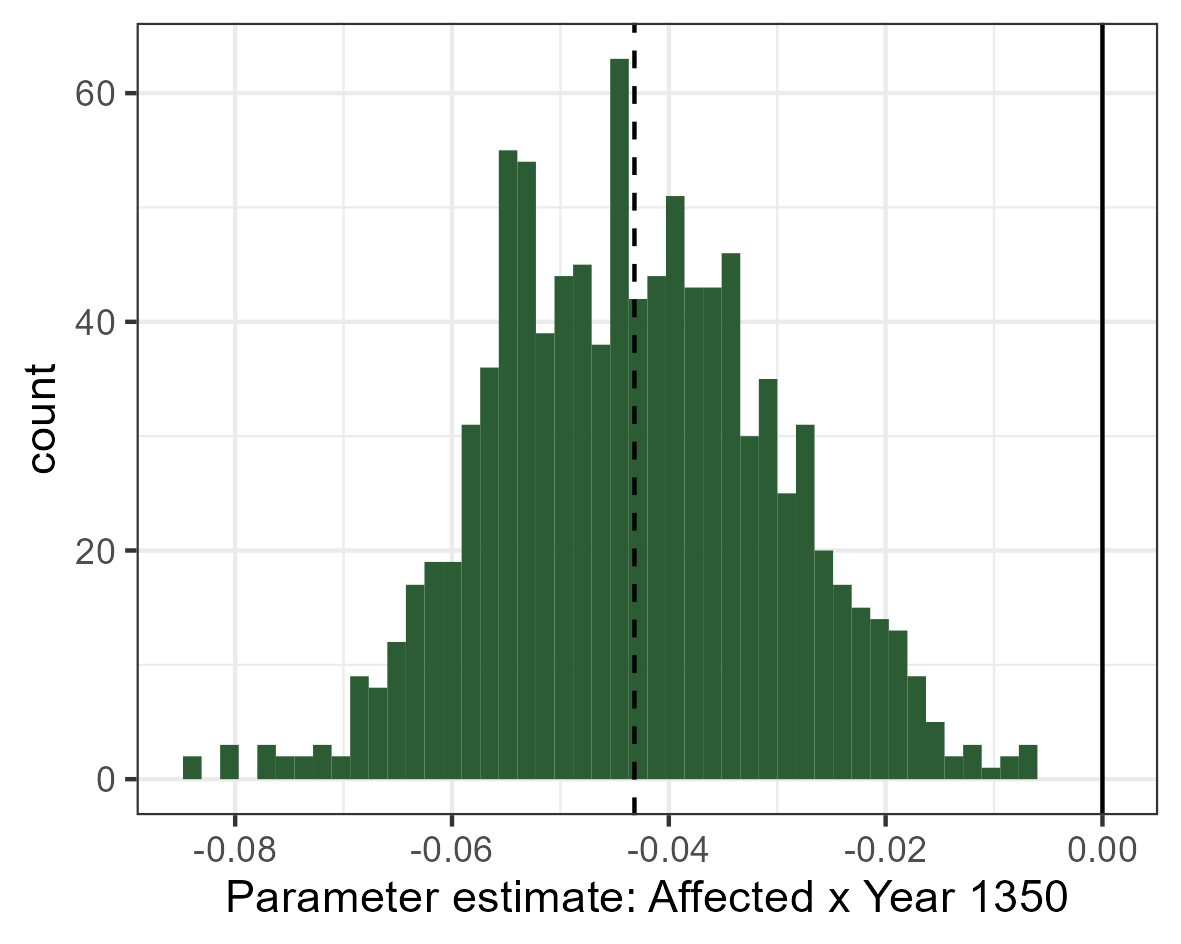
\includegraphics[width=\textwidth]{Plots/Regression_plots/arch_MA_buildings_boot_norm.png}
    \end{subfigure}
    \hfill
    \begin{subfigure}[b]{0.45\textwidth}
        \centering
        \caption{\label{fig:distri_d} Buildings: Dummy approach}
        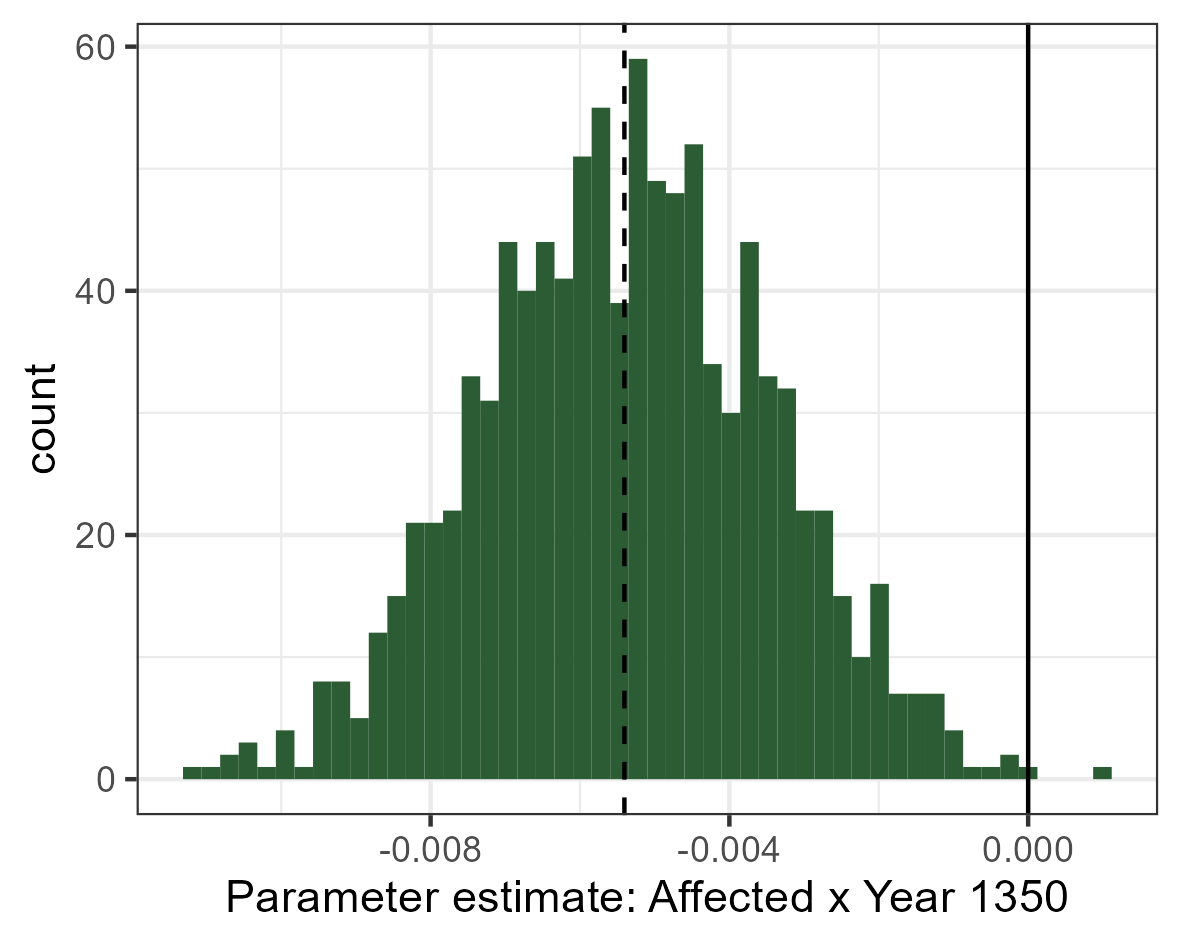
\includegraphics[width=\textwidth]{Plots/Regression_plots/arch_dummy_buildings_boot_norm.png}
    \end{subfigure}
    \label{fig:arch_reg_boot1}
\end{figure}


\begin{figure}[h!]
    \centering
    \caption{Archaelogical results (matched sample)}
    \begin{subfigure}[b]{0.45\textwidth}
        \centering
        \caption{\label{fig:arch1a} Coins: Market access approach}
        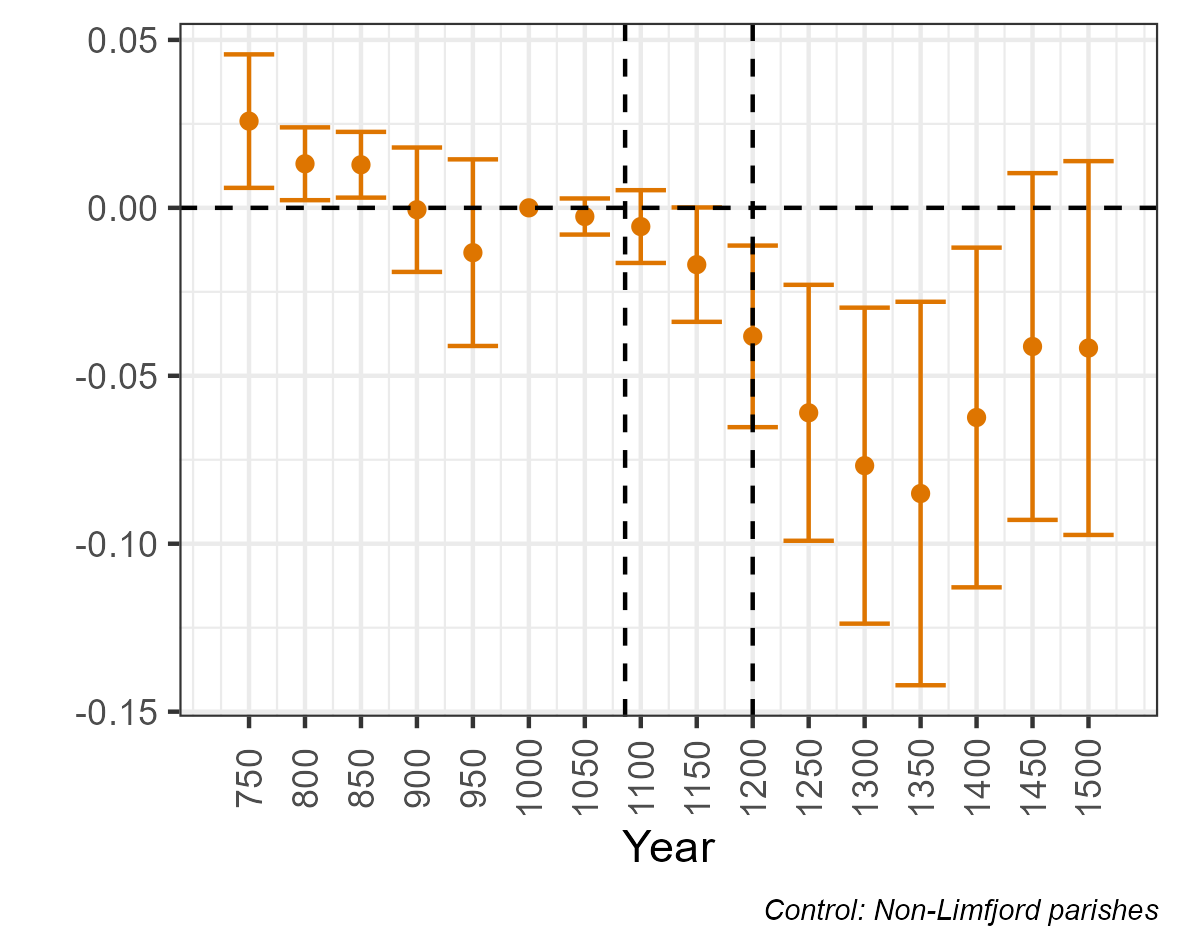
\includegraphics[width=\textwidth]{Plots/Regression_plots/arch_MA_coins_matched_norm.png}
    \end{subfigure}
    \hfill
    \begin{subfigure}[b]{0.45\textwidth}
        \centering
        \caption{\label{fig:arch1b} Coins: Dummy approach}
        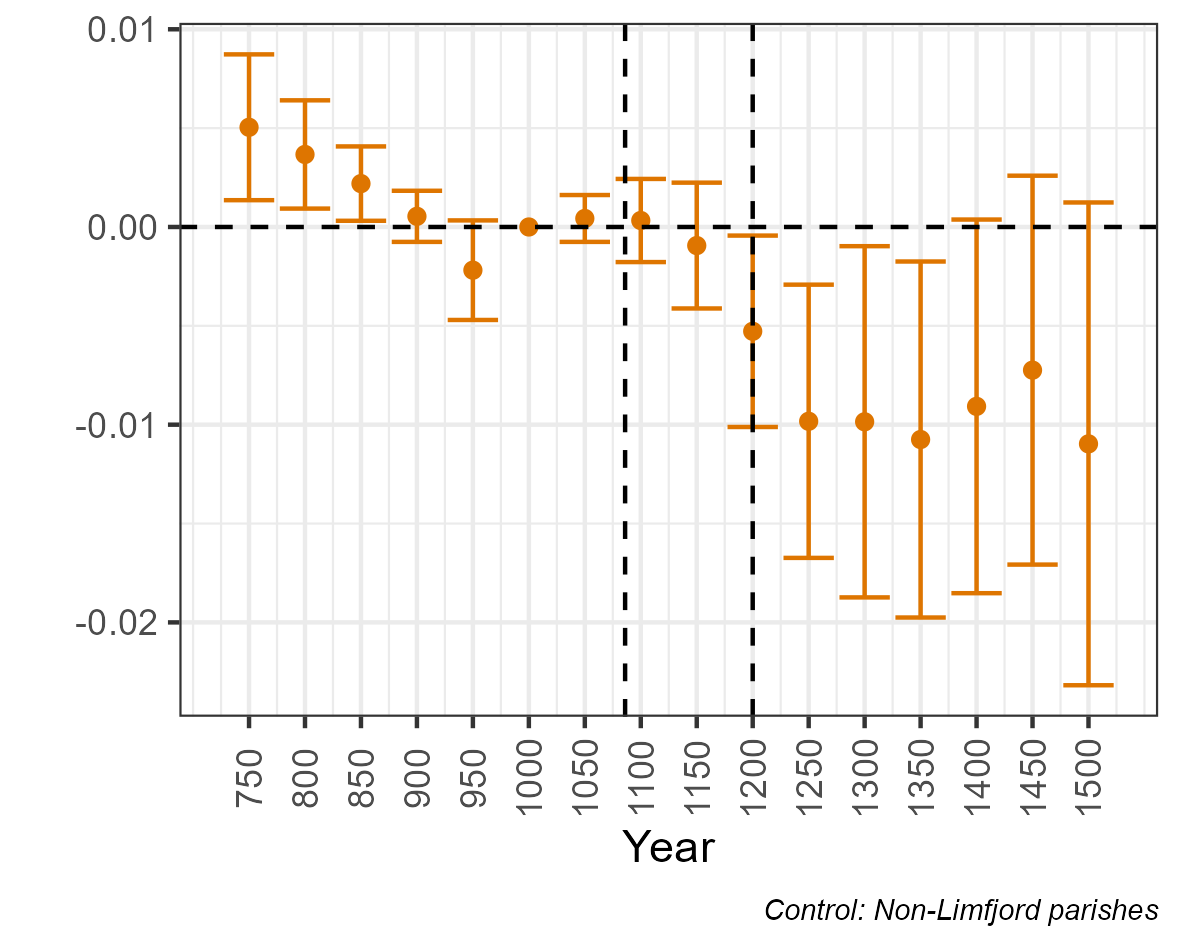
\includegraphics[width=\textwidth]{Plots/Regression_plots/arch_dummy_coins_matched_norm.png}
    \end{subfigure}
    \vspace{0.45cm}
    \begin{subfigure}[b]{0.45\textwidth}
        \centering
        \caption{\label{fig:arch1c} Buildings: Market access approach}
        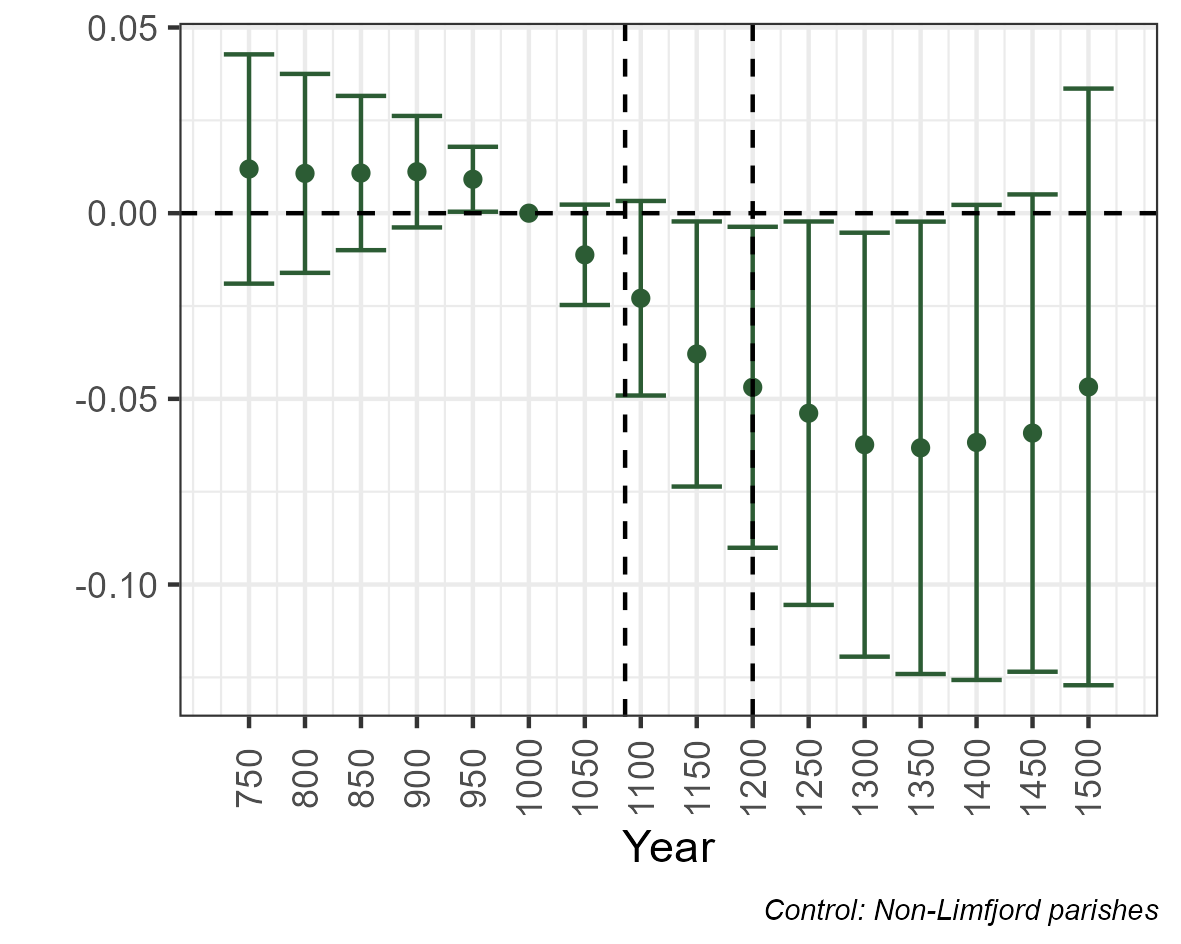
\includegraphics[width=\textwidth]{Plots/Regression_plots/arch_MA_buildings_matched_norm.png}
    \end{subfigure}
    \hfill
    \begin{subfigure}[b]{0.45\textwidth}
        \centering
        \caption{\label{fig:arch1d} Buildings: Dummy approach}
        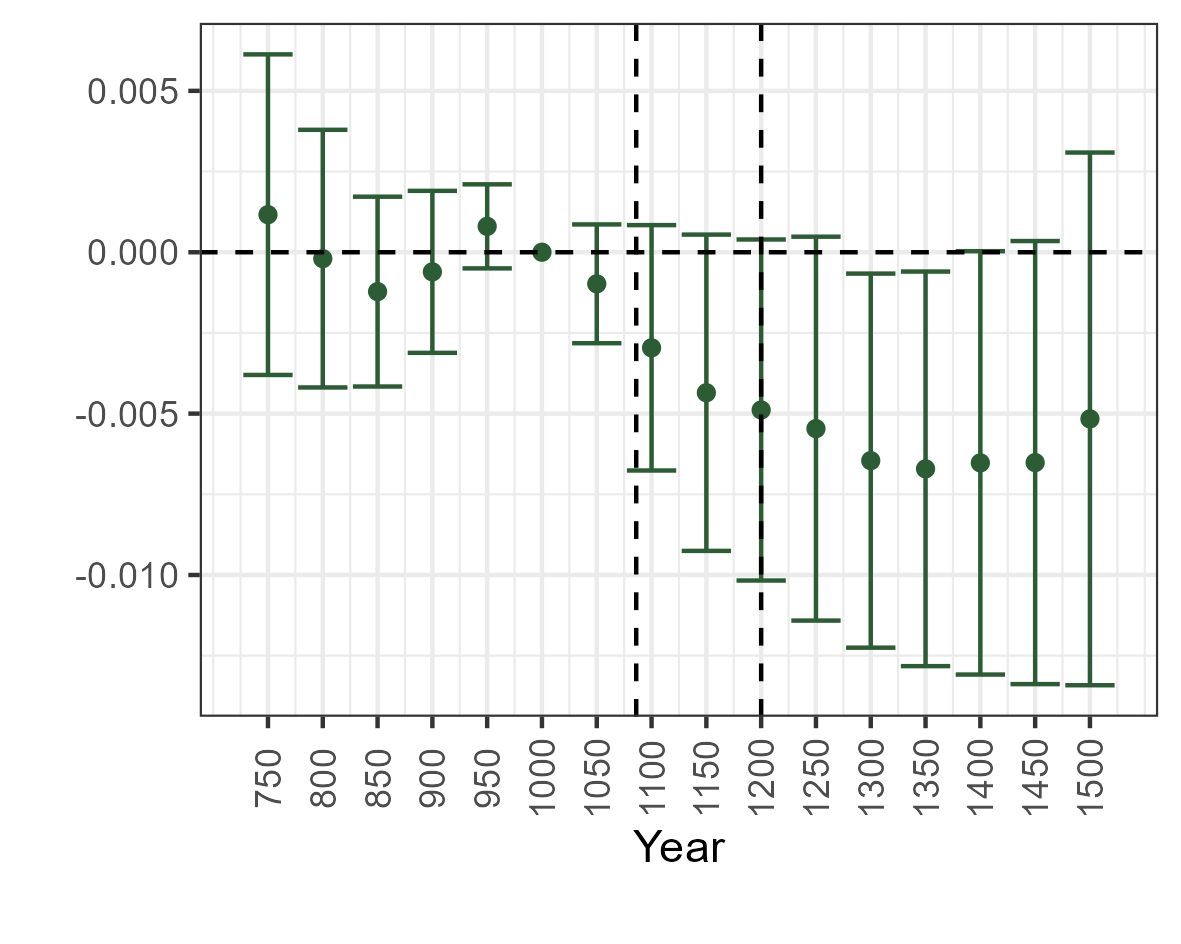
\includegraphics[width=\textwidth]{Plots/Regression_plots/arch_dummy_buildings_matched_norm.png}
    \end{subfigure}
    \label{fig:arch_reg2}
\end{figure}


\begin{figure}[h!]
    \centering
    \caption{Distribution of parameter estimates in 1350  (matched sample)}
    \begin{subfigure}[b]{0.45\textwidth}
        \centering
        \caption{\label{fig:distri_a} Coins: Market access approach}
        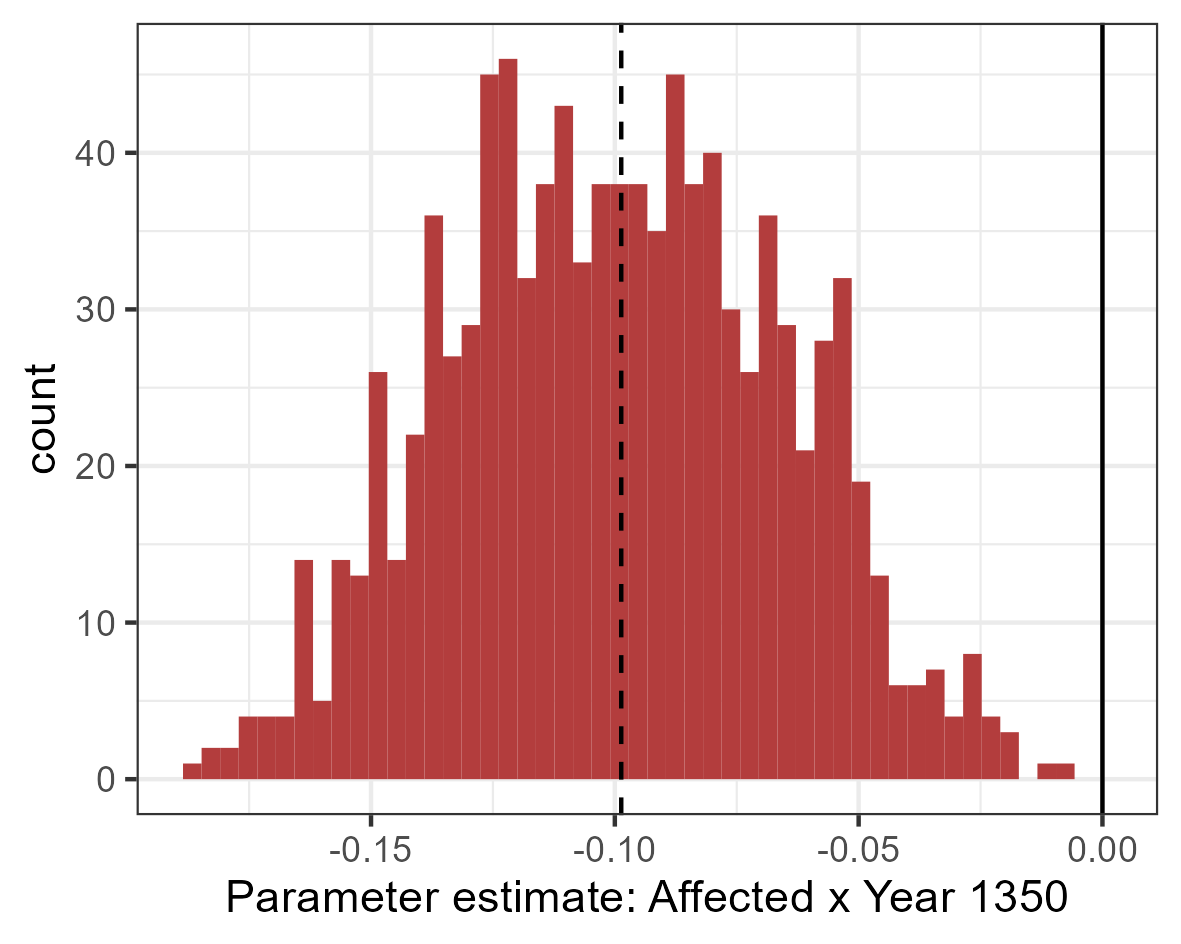
\includegraphics[width=\textwidth]{Plots/Regression_plots/arch_MA_coins_matched_boot_norm.png}
    \end{subfigure}
    \hfill
    \begin{subfigure}[b]{0.45\textwidth}
        \centering
        \caption{\label{fig:distri_b} Coins: Dummy approach}
        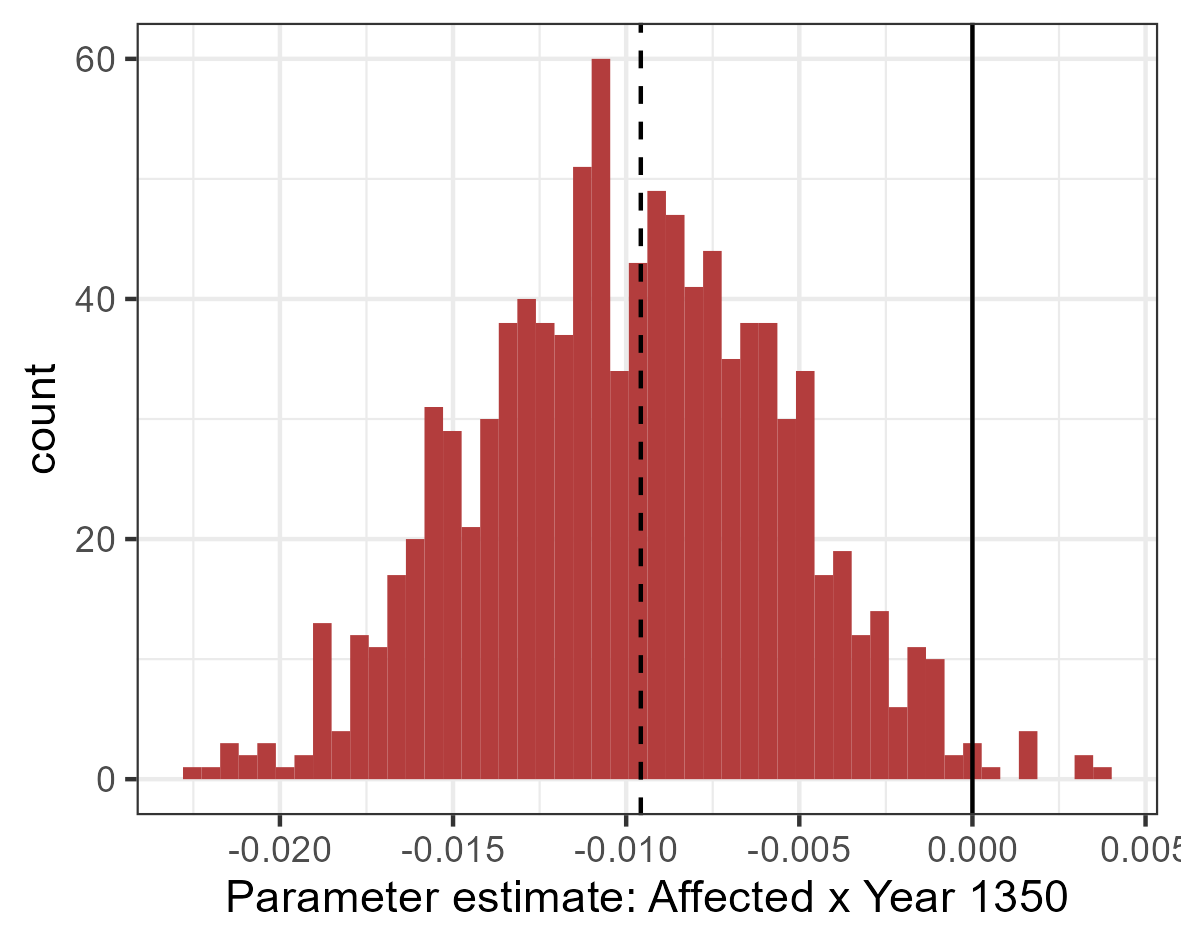
\includegraphics[width=\textwidth]{Plots/Regression_plots/arch_dummy_coins_matched_boot_norm.png}
    \end{subfigure}
    \vspace{0.45cm}
    \begin{subfigure}[b]{0.45\textwidth}
        \centering
        \caption{\label{fig:distri_c} Buildings: Market access approach}
        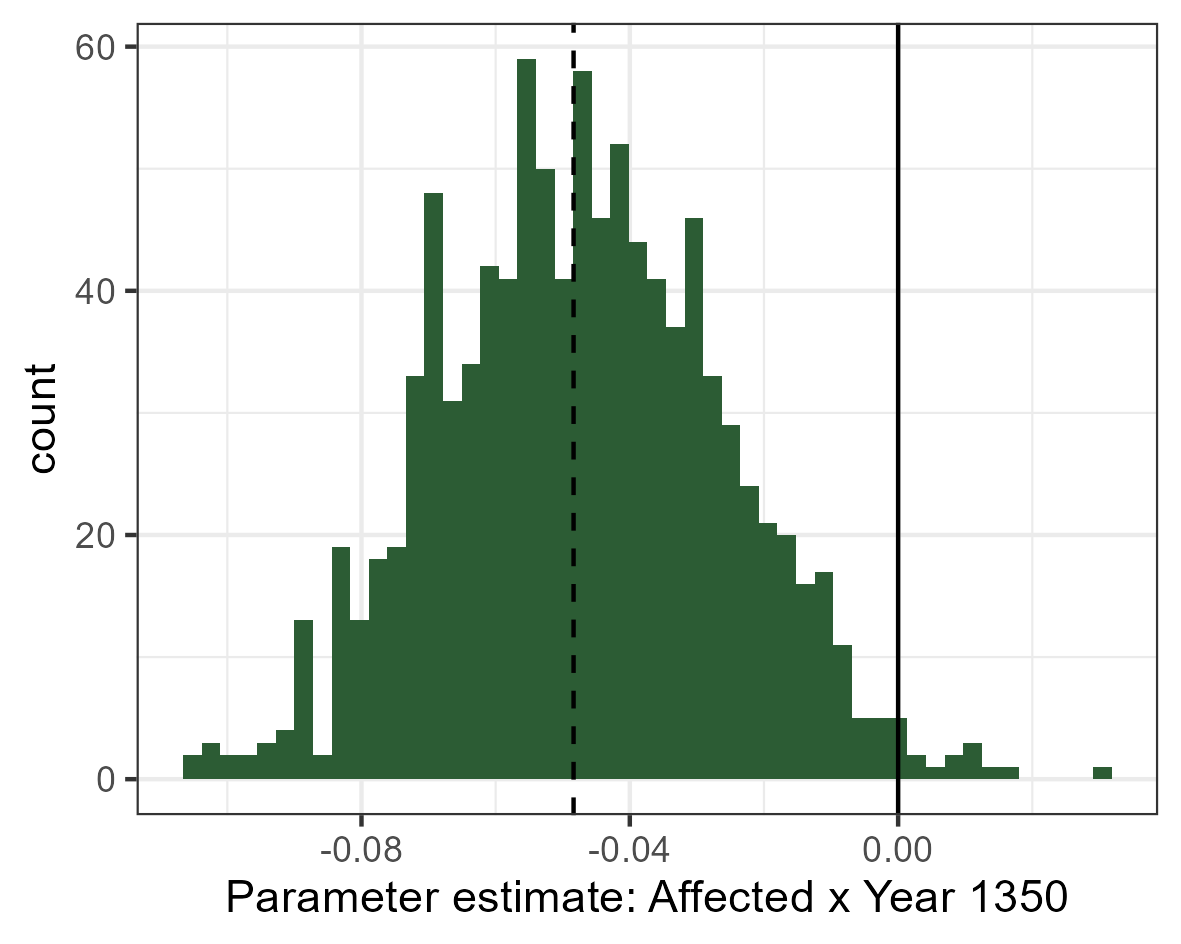
\includegraphics[width=\textwidth]{Plots/Regression_plots/arch_MA_buildings_matched_boot_norm.png}
    \end{subfigure}
    \hfill
    \begin{subfigure}[b]{0.45\textwidth}
        \centering
        \caption{\label{fig:distri_d} Buildings: Dummy approach}
        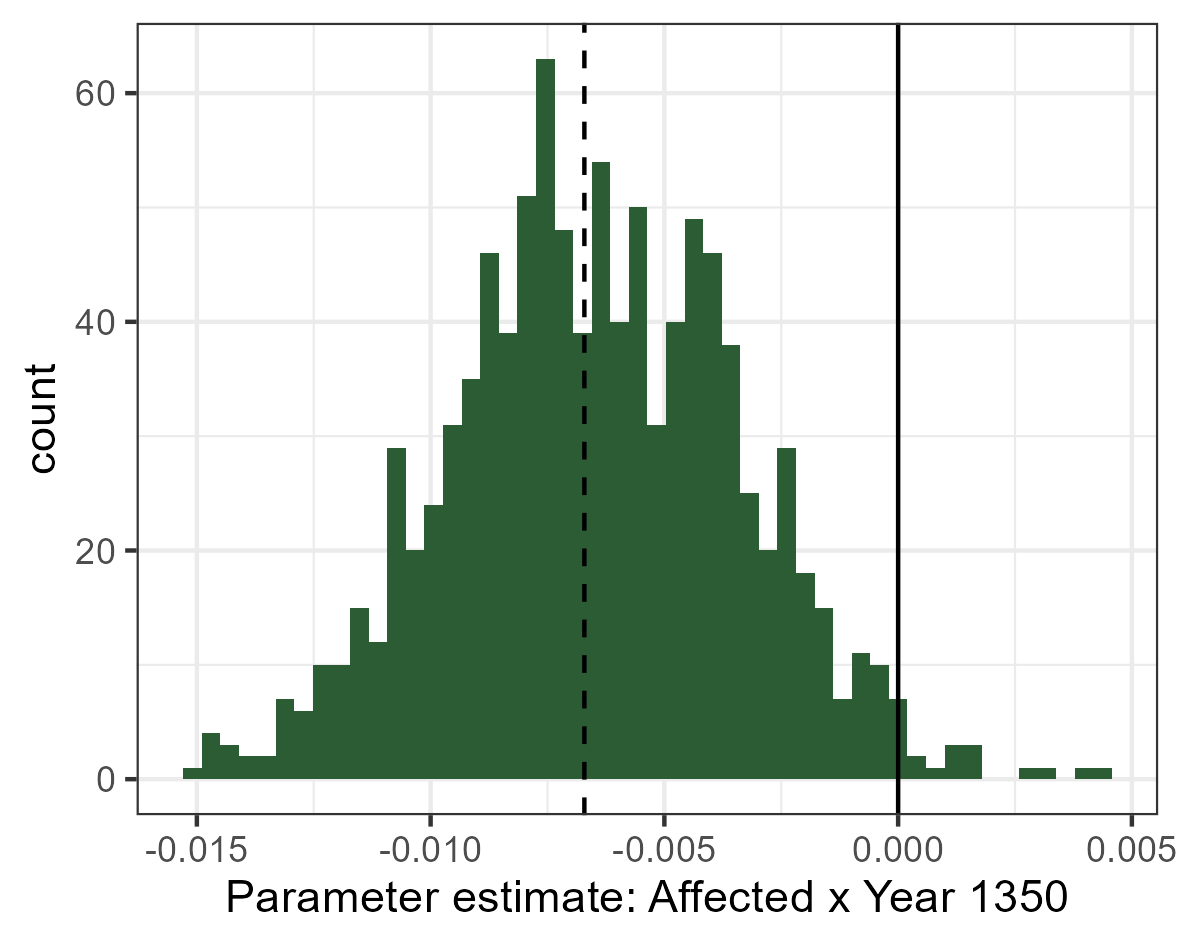
\includegraphics[width=\textwidth]{Plots/Regression_plots/arch_dummy_buildings_matched_boot_norm.png}
    \end{subfigure}
    \label{fig:arch_reg_boot2}
\end{figure}


\bibliographyannex{references}



\end{appendices}